\documentclass[a4paper, 12pt]{scrbook}

%%%------------------%%%
%%%  load the design %%%
%%%------------------%%%
%%%%% ------------------------------------------------%%%%%
%%%%% graphic engine
%%%%% ------------------------------------------------%%%%%
%% Dual Mode
%%
%% Put the pic in the './images' folder. Use the Makefile
%% to convert the images to eps and pdf files. Then
%% the needed pic are selected automaticly by the
%% selected engine (pdf or eps)
%%
\usepackage{graphicx}
\graphicspath{{images_pdf/},{images_eps/}}
%\usepackage{chicago}
\usepackage{amsmath}
\usepackage{subfig}

%\usepackage{psfig}
%\usepackage{fullpage}
%%% EPS only mode
% \usepackage[final]{graphicx}
% \DeclareGraphicsExtensions{.eps}
% \graphicspath{{images_eps/}}
%%
%%% PDF only mode
%\usepackage[final]{graphicx}
%\DeclareGraphicsExtensions{.pdf}
%\graphicspath{{images_pdf/}}
%%%%% ------------------------------------------------%%%%%


%%%%% ------------------------------------------------%%%%%
%%%%% font
%%%%% ------------------------------------------------%%%%%
%\usepackage{type1cm}

%(Times Roman) verwenden (veraltet, durch die folgenden ersetzt)
%\RequirePackage{times}

\RequirePackage{mathptmx}
\RequirePackage[scaled=.90]{helvet}
\RequirePackage{courier}

% Set fonts types for text ...
%\renewcommand{\rmdefault}{phv}  % Helvetica for roman type as well as sf
%\renewcommand{\ttdefault}{pcr}  % use Courier for fixed pitch, if needed

\def\fontdefault{phv} % use let or phv

%% set the default font
%%--------------------------
% uerschriften formatieren ...
\usepackage{caption}
\renewcommand\sfdefault{\fontdefault }
\renewcommand\familydefault{\sfdefault}
\renewcommand{\captionfont}    {\fontfamily{\fontdefault}\selectfont \sffamily}
\setkomafont{pagenumber}       {\fontfamily{\fontdefault}\selectfont \sffamily}
\setkomafont{caption}          {\fontfamily{\fontdefault}\selectfont \sffamily}
\renewcommand{\sectfont}       {\fontfamily{\fontdefault} \bfseries \sffamily}


%% Set Region
\usepackage[english]{babel}
\usepackage[utf8x]{inputenc}

\usepackage[Sonny]{fncychap}

\usepackage{listings}

%%%%% ------------------------------------------------%%%%%
%%%%% Page layout
%%%%% ------------------------------------------------%%%%%

%% Set length parameter to A4
%\usepackage{a4}

%----------------------------------------------------------
% Change page size
%----------------------------------------------------------
%\addtolength{\textwidth}{2cm}
%\addtolength{\textheight}{2cm}
%\addtolength{\oddsidemargin}{-1.0cm}
%\addtolength{\evensidemargin}{-1.0cm}
%\addtolength{\topmargin}{-1.5cm}

% \addtolength{\textwidth}{1cm}
% \addtolength{\textheight}{1cm}
% \addtolength{\oddsidemargin}{-1.0cm}
% \addtolength{\evensidemargin}{-1.0cm}
% \addtolength{\topmargin}{-0.5cm}

\usepackage[right       = 3.0cm,
            left        = 3.0cm,
            top         = 3.5cm,
            bottom      = 3.5cm,
            headheight  = 1.2cm,
            headsep     = 0.5cm,
            foot        = 1.0cm,
            footskip    = 0.8cm]{geometry}
%% Header
\usepackage{fancyhdr}
\pagestyle{fancy}


%\usepackage{epstopdf}

% \renewcommand{\sectionmark}[1]{\markright{\thesection\ #1}}
% \fancyhf{}
% \fancyhead[LE,RO]{\bfseries\thepage}
% \fancyhead[LO]{\bfseries\rightmark}
% \fancyhead[RE]{\bfseries\leftmark}
%
% \renewcommand{\headrulewidth}{0.5pt}
% \addtolength{\headheight}{0.5pt}
% \fancypagestyle{plain}{%
%    \fancyhf{}
%    \fancyfoot[C]{\bfseries \thepage}
%    \fancyhead{}%get rid of headers on plain pages
%    \renewcommand{\headrulewidth}{0pt} % an the line
% }
%
% \setlength{\parindent}{0in}
% \let\margin\marginpar
% \newcommand\myMargin[1]{\margin{\raggedright\scriptsize #1}}
% \renewcommand{\marginpar}[1]{\myMargin{#1}}
%


% create header and footer
%--------------------------
\fancypagestyle{body}
{
    \fancyhf{}
    \fancyhead[RO,LE]{\nouppercase{\rightmark} \vspace{2mm} \hrule}
    \fancyfoot[RO,LE]{\hrule \vspace{2mm} \thepage }
    \fancyfoot[LO,RE]{ \vspace{2mm} Daniel Aschwanden }
    \renewcommand{\footrulewidth}{0pt}
    \renewcommand{\headrulewidth}{0pt}
}

\fancypagestyle{foot}
{
    \fancyhf{}
    \fancyhead[RO,LE]{\vspace{2mm} \hrule}
    \fancyfoot[RO,LE]{\hrule \vspace{2mm} }
    \renewcommand{\footrulewidth}{0pt}
    \renewcommand{\headrulewidth}{0pt}
}

\fancypagestyle{plain} % first page of chapter
{
    \fancyhf{}
    \fancyhead[RO,LE]{\hrule}
    \fancyfoot[RO,LE]{\hrule \vspace{2mm} \thepage }
    \fancyfoot[LO,RE]{\hrule \vspace{2mm} Daniel Aschwanden }
    \renewcommand{\footrulewidth}{0pt}
    \renewcommand{\headrulewidth}{0pt}
}
% configure layout
%--------------------------
\usepackage{titlesec}

\parindent0mm
\parskip2mm
\titlespacing{\section}         {1pt}{*2}{*1}
\titlespacing{\subsection}      {1pt}{*2}{*0}
\titlespacing{\subsubsection}   {1pt}{*2}{*0}


%%%%% ------------------------------------------------%%%%%
%%%%% My Commands
%%%%% ------------------------------------------------%%%%%
\newcommand{\clearemptydoublepage}{\newpage{\pagestyle{empty}\cleardoublepage}}

\def\fig{Fig. }


%%------------------Unknown things ... ------------------%%

%\usepackage{float}
%\usepackage{longtable}

\usepackage{verbatim}
\usepackage{listings}
\usepackage{url}
%\usepackage{hyperref}
%\usepackage{varioref}

% The paralist package provides new list environments for itemized, description, and enumerated lists. With the package, lists can be typeset within paragraphs, as paragraphs in themselves, and in a compressed format. The package allows adjustment of the space between list items in the compressed format. The package also provides arguments for formatting labels in most of the list environments. The package incudes a configuration (.cfg) file that makes standard list environments typeset as if they were the compressed list environments defined by the package. Although the .cfg file isn't part of the default package, the package allows adding a .cfg file. The package may conflict with the babel package.
%\usepackage{paralist}

%\usepackage{psfig}
%\usepackage{url}

%The portland package implements changing from portrait to landscape orientation and back within your SWP or SW document. No special drivers are required, but you may need to change the orientation settings for your printer so that your document prints properly. If you have a single page with an orientation different from that of the rest of the document, you may need to print it separately after changing the printer settings accordingly.

%\usepackage{portland}
%\usepackage{lscape}
%%-lpr \usepackage{verbatim}
%\usepackage{moreverb}

% Write draft on pages ...
%\usepackage[first,bottomafter,light,dvips]{draftcopy}
%\draftcopyName{Draft v0.1}{120}

% ????
%\def\tenrm{\fontsize{10}{12}\normalfont\rmfamily\selectfont}
%\def\BibTeX{{\rmfamily B\kern-.05em{\scshape i\kern-.025em b}\kern-.08em \TeX}}



%\newcommand{\?}{\discretionary{/}{}{/}}
%\newcommand{\liter}[0]{/home/ruf/Lib/Bibl/}
%\newcommand{\fref}[1]{\mbox{Figur~\ref{#1}}}

\usepackage{amsthm}
%\theoremstyle{definition}
\theoremstyle{plain}
\newtheorem{defn}{Definition}[chapter]

%\hyphenation{Lukas not-to-hyphen-else-where}

% \newcommand{\Appendix}[2][?]
% {
%  \refstepcounter{section}
%  \addcontentsline{toc}{appendix}
%  {
%    \protect\numberline{\appendixname~\thesection} %1
%  }
%  {
%    \flushright\large\bfseries\appendixname\ \thesection\par
%    \nohypens\centering#1\par
%  }
%  \vspace{\baselineskip}
% }



%\newcommand\WARN{\myMargin{WARNING}}
%\newcommand\FIX{\myMargin{FIX}}
%\newcommand\UNCLEAR{\myMargin{NOT CLEAR}}
%\newcommand\PROBLEM{\myMargin{PROBLEM}}
%\newcommand\CHECK{\myMargin{CHECK}}
%\newcommand\NEW{\myMargin{NEW}}
%\newcommand\NOTE{\myMargin{NOTE}}
%\newcommand\CHANGE{\myMargin{CHANGE}}
%\newcommand\REMARK{\myMargin{REMARK}}
%\newcommand\THINK{\myMargin{REALLY}}


%\usepackage{config}
\usepackage{pdflscape} 
\usepackage{algorithm}
\usepackage{algorithmic}
\usepackage[longnamesfirst,sort,square]{natbib}

%\usepackage{apacite}
\usepackage{hyperref} 
\usepackage[colorinlistoftodos]{todonotes} 
\usepackage{amsmath}
\usepackage{multirow} 
\usepackage{color} 
\usepackage{textcomp}

% load glossaries after hyperref => links not clickable!
\usepackage[acronym,nonumberlist]{glossaries}


\begin{document}

\frenchspacing \sloppy 

\parskip1ex

\pagestyle{body}

% Title page


%!TEX root = ./main.tex
\begin{titlepage}
	\begin{center}
		\begin{figure}
			[!t] 
			
\includegraphics[width=
			\textwidth]{images/TIKETHhdr.eps} 
		\end{figure}
	\end{center}
	
	\vspace{2mm} \textbf{Daniel Aschwanden}\\
	asdaniel@ee.ethz.ch\\
	07-907-769
	\vspace{2mm}
	
	{\Huge 
	\begin{flushleft}
		Who turned off the Internet?\\
		\LARGE Mining Temporary
		Unreachability 
	\end{flushleft}
	} \vspace{3mm} \centering
	\includegraphics[height=8cm]{images/events/2010_03_25/bgp_log_Set_var_0_1_stab_9_vts_2.eps}
	\vspace{3mm}
	
	Master's Thesis MA-2012-11\\
	April 2012 -- October 2012\\
	
	\vspace{5mm} 
	\begin{tabular}
		{l p{0.3 
		\textwidth} l} \textbf{Advisors:} &&
		\textbf{Supervisor:} \\
		Dominik Schatzmann && Prof. Dr. Bernhard Plattner\\
		Dr. Bernhard Ager && \\
	\end{tabular}
	
	\vspace{8mm} 
	\raggedleft 
	\begin{tabular}
		{rcl} Communication Systems Group&--&
		CSG\\
		Computer Engineering and Networks Laboratory&--&TIK\\
		Department of
		Information Technology and Electrical Engineering&--&ITET\\
		Swiss Federal
		Institute of Technology&--&ETH\\
	\end{tabular}
\end{titlepage} \cleardoublepage

\setcounter{page}{1} 
\pagenumbering{roman}

% Abstract


%!TEX root = ./main.tex
%%%%%%%%%%%%%%%%%%%%%%%%%%%%%%%%%%%%%%%%%%%%%%%%%%%%%%%%%%%%%%%%%%%%%%%%%%%%%%%
%%%%%%%%%%%   How to write an abstract  [1]       %%%%%%%%%%%%%%%%%%%%%%%%%%%%%
%%%%%%%%%%%%%%%%%%%%%%%%%%%%%%%%%%%%%%%%%%%%%%%%%%%%%%%%%%%%%%%%%%%%%%%%%%%%%%%
%
% ----------------------------------------------------------
% Goal:
%  1. ... "selling" your work
%  2. ... "selling" your work
%  3. ... "selling" your work
%
% ----------------------------------------------------------
% Checklist:
%
% Motivation:
% - Why do we care about the problem and the results?
% - Importance of your work, the difficulty of the area,
%   and the impact it might have if successful.
%
% Problem Statement:
% - What problem are you trying to solve?
% - What is the scope of your work ?
%
% Approach:
% - How did you go about solving or making progress on the problem?
% - simulation, analytic models, prototype construction?
%
% Results:
% - What's the answer?
% - is so many percent faster, cheaper, smaller, or otherwise better than something else
% - in numbers
% - talk about orders-of-magnitude improvement not small improvements!!!
%
% Conclusions:
% - What are the implications of your answer?
%
% Keywords:
% - ask your supervisor ...
%
%---------------------------------------------------------%
% Limits:
% - Word count limitation: 150 to 200
%
% [1] Philip Koopman, Carnegie Mellon University, 2007
%     How to Write an Abstract
%     http://www.ece.cmu.edu/~koopman/essays/abstract.html
%     10. Sept. 2007
%----------- FORMAT -----------------------------------------------------------
\clearpage \null 
\vfil 
\begin{center}
	\textbf{Abstract} 
\end{center}

Due to commonly occurring losses of the end-to-end reachability of the Internet, 
many different approaches of detecting these outages have been proposed. 
Although, most of them rely on control-plane information or active probing 
measurements, and are thus not suitable for practical usage. In contrast, the 
fully passive approach FACT is able to reliably track remote connectivity 
issues. 
However, network services have different reachability characteristics and are 
partially designed to be temporary unreachable. This different reachability 
characteristics of connection endpoints introduces some noise in the results of 
FACT. By detecting, monitoring and characterizing network services by their 
visibility, popularity and stability, an adjusted FACT mitigates those event 
detection noise by an order of magnitude. Furthermore, the event visibility is 
further improved by accounting only traffic towards these stable network 
services, hence the outage detection is further enhanced. 

\vspace{10em} 
\begin{center}
	\textbf{network outage detection, network service classification} \par 
\end{center}

%----------- FORMAT -----------------------------------------------------------
\vfil

\newpage
\clearpage \null 
\vfil 
\begin{center}
	\textbf{Abriss} 
\end{center}

Die häufig auftrettenden Unterbrüche der Internet End-zu-End-Erreichbarkeit 
führten dazu, dass viele verschiedene Ansätze zur Detektion dieser Probleme 
vorgeschlagen wurden. Jedoch verlassen sich die meisten dieser Ansätze auf 
Informationen der Kontrollebene oder erfordern aktive Messungen, weshalb sie 
nicht geeignet sind für den Praxiseinsatz. Im Gegensatz dazu ermöglicht der 
völlig passive Ansatz FACT eine zuverlässige Überwachung und Detektion von 
entfernten Verbinungsproblemen im Internet. Verschiedene Netzwerkdienste haben  
unterschiedliche Erreichbarkeitscharakteristiken und sind zum Teil dafür 
ausgelegt sind, temporär nicht erreichbar zu sein ohne den Netzwerkbenutzer zu 
beinträchtigen. Dies führt dazu, dass FACT zum Teil Probleme erkennt, welche in 
Wirklichkeit keine sind und als eine Art von Rauschen bezeichnet werden können. 
Durch die Detektion, Überwachung und Charakterisierung der Netzwerkdiense kann 
eine angepasste Version von FACT dieses Rauschen um eine Zehnerpotenz 
verkleinern. Im Weiteren sind die Probleme besser sichtbar 
und die Überwachungmöglichkeiten von FACT erweitert worden.

\vspace{10em} 
\begin{center}
	\textbf{network outage detection, network service classification} \par 
\end{center}

%----------- FORMAT -----------------------------------------------------------
\vfil


%
% Preface


%!TEX root = ./main.tex
%\clearpage
%\null
%\vfil
%---------- FORMAT -----------------------------------------------------------
\clearpage 
\begin{center}
	\textbf{Acknowledgments} 
\end{center}

During the creation of this thesis several people supported me. At this place, I would like to thank them.

At first, I am deeply grateful to Dominik Schatzmann and Dr. Bernhard Ager for their support, their great expertise and their patience in explaining me even basics concepts. They always asked the right questions at the right time, thus directing my focus on the important things. During the last half year, they always provided good remarks and excellent advisory -- not only regarding technical aspects. I really enjoyed the discussions and the process of working on this thesis with them. 

Furthermore, I would like to express my sincere gratitude to Prof. Dr. Bernhard Plattner for providing the opportunity to write this thesis in his research group and his excellent remarks. 

In addition, I enjoyed the support of the entire Computer Engineering Group (CSG) in various situations. In particular, I am grateful to Brian Trammell for always providing me the required support regarding the computing infrastructure in an extraordinary pleasant manner. 

Finally, I am very thankful to my close friends for motivating and supporting me in all circumstances.

%---------- FORMAT -----------------------------------------------------------
\vspace{1cm} Daniel Aschwanden 
\vfil

%---------- END -----------------------------------------------------------

%%% GLOSSARY %%%%
%!TEX root = ./main.tex

%%%%%%%%%%%%%%%%%%%%%%%%%%%%%%%%%%%%%%%%%%%%%%%%%%%%%%%%%%%%%%%%%%%%%%%%%%%%%%%%
% GLOSSAR
%%%%%%%%%%%%%%%%%%%%%%%%%%%%%%%%%%%%%%%%%%%%%%%%%%%%%%%%%%%%%%%%%%%%%%%%%%%%%%%%
% control-plane
\newglossaryentry{control-plane}{
	name=control-plane,
	description={}
}

% data-plane
\newglossaryentry{data-plane}{
	name=data-plane,
	description={}
}


\newglossaryentry{osi-mod}{
	name=Open Systems Interconnection Reference Model,
	description={describes the layered architecture of the Internet, standardized by ISO/IEC 7498-1}
}

% NetFlow
\newglossaryentry{netflow}{
	name=NetFlow,
	description={is a network protocol for collecting IP traffic information and was originally developed by Cisco Systems}
}

\newglossaryentry{server socket}{
	name={server socket},
	description={is a socket with a process listening to incoming connections and thus offering a network service.}
	plural={server sockets},
}


%%%%%%%%%%%%%%%%%%%%%%%%%%%%%%%%%%%%%%%%%%%%%%%%%%%%%%%%%%%%%%%%%%%%%%%%%%%%%%%%
% ACRONYMS
%%%%%%%%%%%%%%%%%%%%%%%%%%%%%%%%%%%%%%%%%%%%%%%%%%%%%%%%%%%%%%%%%%%%%%%%%%%%%%%%
% OSI
\newacronym{osi}{OSI}{\Gls{osi-mod}}

% ISP
\newacronym{isp}{ISP}{Internet service provider}

% BGP
\newacronym{bgp}{BGP}{Border Gateway Protocol}
% AS
\newacronym{AS}{AS}{autonomous system}

% SLA
\newacronym{sla}{SLA}{service level agreement}

% IS-IS
\newacronym{is-is}{IS-IS}{Intermediate System to Intermediate System Protocol}

% FACT
\newacronym{FACT}{FACT}{Flow-based Approach for Connectivity Tracking}

% NAT
\newacronym{nat}{NAT}{network address translation}

% CDN
\newacronym{cdn}{CDN}{content distribution networks}

% TCP
\newacronym{TCP}{TCP}{Transmission Control Protocol}

% UDP
\newacronym{UDP}{UDP}{User Datagram Protocol}

% IP
\newacronym{IPv4}{IPv4}{Internet Protocol version 4}
\newacronym{IPv6}{IPv6}{Internet Protocol version 6}

% HTTP, FTP, SSH
\newacronym{HTTP}{HTTP}{Hypertext Transfer Protocol}
\newacronym{FTP}{FTP}{File Transfer Protocol}
\newacronym{SSH}{SSH}{Secure Shell}
\newacronym{NTP}{NTP}{Network Time Protocol}

% P2P
\newacronym{p2p}{P2P}{peer-to-peer}

% DDoS
\newacronym{DDoS}{DDoS}{distributed denial of service}

% SES
\newacronym{ses}{SeS}{server socket}







\makeglossaries
\printglossary
\printglossary[type=\acronymtype]

\tableofcontents

\cleardoublepage

% Content
\pagenumbering{arabic} \setcounter{page}{1}

%!TEX root = ./main.tex
\chapter{Introduction\label{Introduction}}

% Problem: Connectivity problems exist
The end-to-end connectivity of hosts is one of the key services of the Internet. However, even after 40 years of intense engineering efforts, this connectivity is temporally broken for various reasons, such as link or hardware failure \citep{Markopoulou:2008}, mis-configurations \citep{Mahajan:2002}, or natural disasters \citep{Dainotti:2012:EBH,Schulman:2011}. 

% (Centrality Claim) Why do we care: Requires Troubleshooting Tools (TST) to minimize costs
This shows that there is a real need for methods to systematically detect and locate Internet outages of remote autonomous systems, subnets, and even single hosts. This is particularly true for \gls{isp}, because time intensive debugging sessions and the support of customers complaining at the \gls{isp} for unreachable networks are generating costs for the \gls{isp}. Occasionally, a \gls{isp} is even contractually liable for unreachable networks within the scope of a \gls{sla}. Therefore, an automated, ongoing detection and tracking of connectivity issues of the Internet may generate transparent outage information for customers and enables the \gls{isp} to react adequately on a detected reachability problems if possible, for example by changing routes in case of a failure of a transit provider. 

% (What is missing) Introduce the gap that we plan to close: 
Researchers and industrial vendors have proposed various approaches to systematically detect, locate and troubleshoot Internet outages due to the loss of end-to-end reachability. 

% State clearly what is missing
However, most of these approaches rely on \gls{control-plane} information such as \gls{bgp} routing messages or \gls{data-plane} information achieved by active probing. Both approaches are not perfectly suitable for practical usage.
% bash: control plane approaches & active probing approaches
As shown by \citet{Bush:Optometry}, packets in the Internet do not necessarily follow the \gls{control-plane} due to default routes or other secret peering policies. Moreover, connectivity issues imposed by packet filtering cannot be tracked by \gls{control-plane} approaches \citep{Dainotti:2011:ACI}. Besides legal issues, active probing requires the cumbersomeness of target selection and significantly increases the load on Internet infrastructure. Furthermore, there is still no active approach which scales well enough for the entire \gls{IPv6} address space. Moreover, both approaches are unable to track which part of the Internet is currently actively used by their internal clients. This is required to determine the amount of affected internal clients and therefore to assess the urgency of the outage event. For example, as long as a connectivity issue occurs within an unused remote network, the operator can handle this event with low priority and fix more urgent problems first.
To fill this gap, \citet{SchatzmannPAM2011} proposed the fully passive approach called \gls{FACT} relying on flow-level information to identify remote connectivity problems. The basic idea of \gls{FACT} is to match the corresponding outgoing and incoming flow to a bidirectional connection. Then, the remaining unidirectional connections or unresponsive connections are extracted and investigated. 

The detection of an outage is consolidated by aggregating these unresponsive connections to host, network and \gls{AS} level and rating the severity of the events by the number of affected internal users. This consolidation is required to reduce the noise of unresponsive connections caused by scanning or botnets and implies an implicit prioritization of events which affect many internal network users.

\citet{SchatzmanThesis2012} proposed to treat certain types of Internet services differently, because they do not require constant reachability. For example, Skype or BitTorrent applications that are often executed on client machines such as Desktops, Laptops, or Smartphones are likely to be reachable only for a limited time during a day.
This characteristic is caused by the fact that these machines are often disconnected from the network to save power or due to mobility effects. However, this temporal unreachability is not noticed as a problem by end-users. 
Therefore, issues of such client machine based services should not be treated the same way as server machine based services.

Currently, \gls{FACT} does not differentiate the kind of service for tracking connectivity issues. This leads to the problem that client based services which are designed to be temporarily unavailable are in the worst case incorrectly interpreted as network outage. At the moment, \gls{FACT} is dealing with this problem by three different approaches.

Firstly, \gls{FACT} monitors in a first step only traffic towards stable services. At the moment, this is heuristically defined by the traffic going to a remote \gls{TCP} port 80 traffic from an internal client high port, representing the assumption that this kind of traffic is destined for a legitimate and stable web server socket. This approach can be viewed as preselecting only the traffic destined for stable services.  

Secondly, a network is only declared as unreachable if and only if all connection endpoints located in this network are not responding resembling a kind of network based traffic aggregation. 

In addition, a detected network outage is rated by the number of internal users which are affected by this specific outage and thus prioritizing relevant network outages.

\begin{figure}
	[ht] \centering
	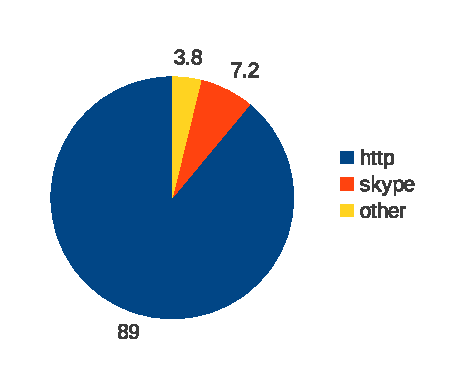
\includegraphics[width=6cm]{images/application_fact_port_80.eps}
	\caption{Application traffic running on TCP port 80 \citep{SchatzmanThesis2012}} 
	\label{fig:tcp_port80}
\end{figure}

However, by performing deep packet inspection \citet{SchatzmanThesis2012} has shown that the heuristic port based traffic preselection is not ideal, since a handful other applications are running on \gls{TCP}  port 80, presumably for firewall avoidance purposes. As shown in figure \ref{fig:tcp_port80}, the most relevant application running on \gls{TCP} port 80 -- besides \gls{HTTP} -- is Skype with a share of $7.2\%$ of all \gls{TCP} port 80 traffic. 

This \gls{TCP} port 80 based Skype traffic yields a completely different reachability characteristic. As shown by \citet{SchatzmanThesis2012}, there is a significantly higher amount of Skype \gls{TCP} port 80 sockets not reachable compared to \emph{normal} web server sockets of \gls{cdn} which is illustrated by figure \ref{fig:skype_traffic}. This exacerbates the reliable detection of network outages. 

\begin{figure}
	[ht] \centering
	\includegraphics[width=12cm]{images/application_fact.eps}
	\caption{Unreachable TCP port 80 sockets differentiated by Skype and CDN application running on these sockets. \citep{SchatzmanThesis2012}} 
	\label{fig:skype_traffic}
\end{figure}

To this end, this thesis proposes a new type of traffic preselection which includes only traffic towards stable and reliable services. This is achieved by selecting traffic based on the past stability and popularity characteristics of remote services instead of the current heuristic port-based traffic preselection.

In detail, remote services are monitored and analyzed on longer time scales so that the deduced statistical information allows the characterization of the services. Consequently, only traffic towards sockets which are characterized as stable are monitored by \gls{FACT}. For example, a remote web server used only by few users that is often unreachable, e.g.,due to testing or resource scarcity, should not be monitored by \gls{FACT}. In contrast, a popular content distribution host that was always reachable in the past is more relevant. 

To sum up, the overall goal of this thesis is to extend \gls{FACT} with a service monitoring and classification functionality to enhance the current rudimentary traffic preselection. In fact, this functionality should allow \gls{FACT} to focus even better on relevant connectivity issues which are related to stable and popular services.


\section{Related Work 
\label{sec:related_work}}
Due to the special interest of research and industrial vendors in the problem, there is a great effort done in the past. 
Generally, the related work with impact on this thesis can be separated into two thematically different topics.
On the one hand, there is a lot of research done in the area of reachability tracking. 
On the other hand, the topic of detecting network services is not only of interest for research and industry, but also for cyber criminals. 
In the following, both areas are briefly covered. 

\subsection{Reachability Tracking}

% Connection Tracking (Active & Passive)
Severe disruptions of the Internet's end-to-end connectivity is not a new phenomenon, there have been connectivity outages since its beginning as research project. 
Despite that the end-to-end connectivity is a very basic service of the Internet, the Internet community has not a deeply founded understanding of the problems that causes its disruption \citep{Bush:Optometry}.
A dominant share of researchers focussed on "pathological behavior related to the address space, e.g., bogon advertisements \citep{Feamster:2005}, prefix hijacking \citep{Zhang:2010}, \gls{bgp} misconfigurations \citep{Mahajan:2002} or \gls{DDoS} attacks \citep{Chen:2001}"\citep{Bush:Optometry}.

Basically, reachability can be viewed from two perspectives: \gls{data-plane} and \gls{control-plane} measurements. \citep{Feamster:2005,Zhang:2010,Mahajan:2002,Chen:2001} are mainly based on \gls{control-plane} information as publicly available BGP data for deducing knowledge about reachability. 
\citet{Bush:Optometry} pointed out that tracking \gls{data-plane} reachability with \gls{control-plane} information is heavily inaccurate due to the effect of secret peering policies, e.g., default routing. 
These allow packets to reach their destination even when a route failed to propagate through the \gls{bgp} system. 
\citet{Bush:Optometry} stated that even very basic \gls{data-plane} measurements
produce better views on reachability than \gls{bgp} observations. 
However, \gls{control-plane} based measurements are not limited to \gls{bgp} data, \citet{Markopoulou:2008} classified failures in a IP backbone network with \gls{is-is} information and tried to characterize these failures by layers as router, optical/link and maintenance. 
To sum up, \gls{control-plane} measurements of reachability are indirect and thus of limited practical usage for systematical reachability tracking approaches.

In contrast, measurements of the \gls{data-plane} are direct and can be more accurate regarding end-to-end connectivity. 
\Gls{data-plane} measurements can be divided into active probes and passive monitoring. 
Whereas active probes generates additional traffic towards the observed address space of the Internet, passive monitoring relies mainly on the traffic of servers and clients of the network or the traffic towards them. 

Active probing is widely used for end-to-end reachability problem detection, ranging from rudimentary debugging tools as ping \citep{PING}, paris traceroute \citep{traceroute} or nmap \citep{Nmap} to highly sophisticated, automated
outage detection tools as Hubble \citep{Katz:2008} or PlanetSeer \citep{Zhang:2004}. 
\citet{Bush:Optometry} pointed out that there exist some important limitations of active probing approaches as filtered packets by firewall and \gls{nat} devices or suboptimal routing which result in intermittent problems as packet rerouting.
Furthermore, there is no active probing technique known which is able to record the return-path in addition to the forward-path which can be extracted for example with traceroute probes. 
It is not generally true to deduce that forward-path reachability implies return-path reachability as well, since there may be intermittent problems caused for example by suboptimal routing \citep{Bush:Optometry}.

% Pingin' in the rain (Schulman/Spring)
\citet{Quan12a} implemented an Internet outage detection engine which is able to actively probe a representative part of the Internet and correlate outage events with \gls{control-plane} information. 
This is achieved by a sophisticated target selection approach. 
However, this approach is avoiding some of the drawbacks of active probing as blockage by firewalls and \gls{nat} devices by clearly state that they are able to track the "analyzable" \gls{IPv4} address space of the Internet which represents the space which is answering on their active probes.
The future scalability of this approach -- especially with respect to \gls{IPv6} -- is questionable. 

%_--- PASSIVE --
Besides the big amount of different approaches using active probing, only few approaches are using passive monitoring for reachability tracking. 
\citet{Dainotti:2011:ACI} presented an approach for an in-depth analysis of connectivity outages caused by political censorship by combining observations from \gls{bgp} data, \gls{data-plane} information as backscatter measurements of the UCSD network telescope, and active probing measurements from the Archipelago Measurement Infrastructure. 
Remarkable is their approach of (passively) monitoring of the unsolicited \gls{data-plane} traffic that shed light on Libya's attempts on deploying packet filters for enforcing the Internet censorship. 
They concluded that this unsolicited and unwanted traffic captured by network telescopes may "illuminate many different types of macroscopic events, including but not limited to broad-scale packet-filtering-based censorship, which is not observable by \gls{bgp} data."\citep{Dainotti:2011:ACI}.

% evtl iatmon noch..
%\citet{SchatzmannPAM2011} aim to detect reachability problem by passively monitoring \gls{data-plane} measurement and aggregate unresponsive connection attempts on network- and AS-level.
\subsection{Service Detection} 

% Service Detection (Active & Passive, completeness vs. scalability / importance)
The discovery and characterization of services in the Internet is most successfully done on a massive scale, ironically not by researchers but by worms and other malware\citep{Chen:2007}. 
Generally, service detection methods can mainly be grouped into two approaches: passive monitoring and active probing. 
As \citet{Bartlett07b} pointed out, active probing is able to detect all visible and scannable services, which is thus invasive and legally constrained. 
On the other hand, passive monitoring is able to find transient services, but fails to detect idle services. 
In their work, they compared the "accuracy of passive and active approaches to service discovery and showed that they are complimentary"\citep{Bartlett07b}. 
They concluded that best results are achieved by combining a long lasting passive monitoring with multiple active scans, thus forming a hybrid approach\citep{Bartlett07b}. 

\citet{Leonard:2010} developed an Internet-wide service scanner called IRLscanner. 
They designed their scanner to maximize politeness to remote networks by smartly choosing adequate scanning rates. 

% Webster active / passive
\section{Contribution 
\label{sec:contribution}}
This master thesis contributions are the following: 
\begin{itemize}
	\item qualitative analysis of remote server sockets found by a passive approach based on \citet{Schatzmann:Mining,Schatzmann:Dissection, Schatzmann:Tracing} regarding their characteristics of stability, visibility and popularity.
	\item synthesis of the findings of this characterization for enhancing the traffic selection for tracking remote connectivity issues based on the approach of \citet{SchatzmannPAM2011}.
\end{itemize}

\section{Outline
\label{sec:outline}}



\todo{Write me at last..}


%!TEX root = ./main.tex
\chapter{Background\label{Background}}

\section{FACT}



% Implementation


%!TEX root = ./main.tex
\chapter{Approach
\label{chapter:approach}}

\section{Methodology
\label{section:methodology}}

To achieve the goal of enhancing the traffic preseleciton of FACT with
knowledge about the past stability and popularity characteristics, the following
three steps are planned for extending FACT as illustrated in figure
\ref{fig:FACT}.
\begin{figure}
	[ht] \centering
	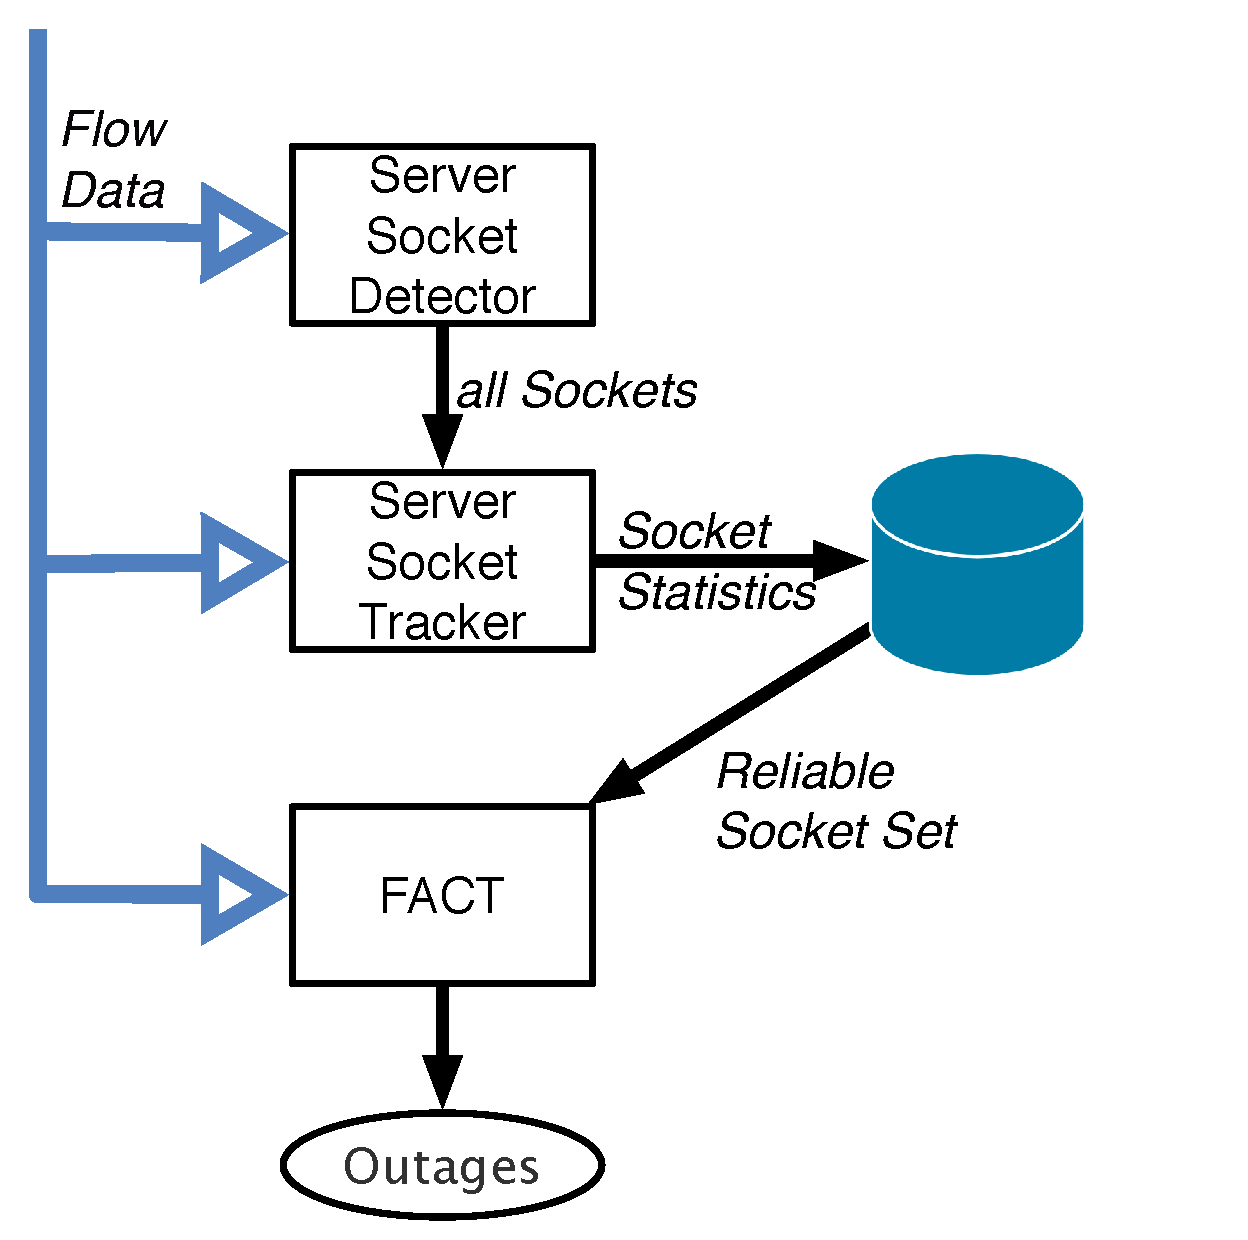
\includegraphics[width=8.5cm]{images/Approach_blockdiagram.eps}
	\caption{Interactions of new components with FACT} 
	\label{fig:FACT} 
\end{figure}

In a first step, a server socket detector is implemented. The challenge of the
server socket detection lies in the fact that the netflow data does not provide
enough precise timing information to determine which flow is originated from the
client and thus determine the server's socket. Therefore, the server socket
detection is achieved by the assumption that server sockets act as concentrators
in the sense that several clients have connections to the identical server
socket and bases on the work shown in
\cite{Schatzmann:Dissection,Schatzmann:Mining,Schatzmann:Tracing} and is
discussed in more detail in section \ref{section:socket_detection}.

Secondly, the previously detected server sockets are continually monitored and
especially the successful and unsuccessful connection attempts are recorded by
the server socket tracker.
Furthermore, these information are used to update the statistical information of
visibility, popularity and stability. Section \ref{section:socket_tracking}
covers this step in detail.

In a third step, the number of server sockets have to be reduced and selected
such that FACT is able to use these sockets for outage tracking. In particular,
the server sockets coverage of the Internet address space has to be optimized.
It makes no sense to select only the most popular sockets if they are all
located in the same /24 network.

Finally, FACT has to be adopted to optimally use the preselected and rated
server sockets for prioritizing relevant connectivity issues by reducing outage
alerts based on single host outages of unstable services.

%%%%%%%%%%%%%%%%%%%%%%%%%%%%%%%%%%%%%%%%%%%%%%%%%%%%%%%%%%%%%%%%%%%%%%%%%%%%%%%%
\section{Data
\label{section:data}}

This thesis relies on data collected at \citet{switch}, the Swiss National 
Research and Education Network (NREN). Mainly government institutions, 
universities, research labs are connected to the internet by \citet{switch}\citep{Schatzmann:Mining}.

The \citet{switch} network is with approximately 250'000 network users in 2010 comparable with a mid sized ISP. Currently, there are around 2.4 million IPv4 addresses, a /32 IPv6 and a /40 IPv6 network announced via BGP\citep{Schatzmann:Tracing}.

\citet{switch} is capturing flow level data at all external interfaces of their border routers by 2003 in form of unsampled NetFlow data -- from 2003-2008 in version 5 and in version 9 after 2008\citep{Schatzmann:Tracing}.
High traffic peak rates of more than 80'000 flows per second, 3 million packets per second and more than 20Gbit/s require hardware-based flow collection cards. TCP flags are not available in the flow level information because of some limitations of these hardware components. The generated flow data is collected and stored at a central data repository.

% briefly describe the Switch network and its topology..
% traffic volume and netflow data unsampled!
% see tech report 338 for numbers and layout?! evtl actual numbers (2012)
%%%%%%%%%%%%%%%%%%%%%%%%%%%%%%%%%%%%%%%%%%%%%%%%%%%%%%%%%%%%%%%%%%%%%%%%%%%%%%%%
\section{Flowbox
\label{section:flowbox}}

Flowbox is a modular flow processing library developed by the Communication Systems Group (CSG) at ETH Zurich. It aims to allow an easy composition of individual flow processing components for common processing tasks. Moreover, it provides an easy interface for developing own components for specialized tasks that rely on other processing components of Flowbox.

Generally, there are two flow data formats, an unidirectional flow (\emph{Flow}) and bidirectional flow (\emph{BiFlow}). A bunch of such flow records are put into containers -- either \emph{FlowContainer} or \emph{BiFlowContainers}. Those containers are then passed to buffers (\emph{FlowContainerBuffer} or \emph{BiFlowContainerBuffer}) interconnecting the individual processing blocks.

These processing blocks can be grouped into the three groups, Flow Reader, Caches, and Filters. The individual blocks which are available by September 2012 are briefly described in the following:

\subsection{Flow Readers}

\subsubsection{NetFlowV5 Parser} 
\subsubsection{NetFlowV9 Parser}
\subsubsection{CSG Flow Parser} 


% configured with internal prefixes, responsible for tagging flows with direction. Setting transit and internal network traffic (in-in) as invalid (filtering away)
\subsection{Caches}
\subsubsection{BiFlowCache} This module is responsible for generating
bidirectional flows from incoming unidirectional flows. This is done by
storing the flows in hash table with a hash key which is identical for incoming
and outgoing flows and thus matching the corresponding reverse flows. For proper operation of the \emph{BiFlowCache}, a properly configured \emph{InOutFilter} is required in front of the BiFlowCache, since it is necessary that the direction of all flows must be tagged either as outgoing or as incoming and that only cross-border flows are processed.

\subsubsection{ConnectionCache}

\subsection{Filters}
\subsubsection{InOutFilter}
\subsubsection{IP Filter} 
\subsubsection{Noise Filter} 
\subsubsection{Fan-Out Filter}





%!TEX root = ./main.tex
\chapter{Of Server Sockets and their Characteristics 
\label{chapter:sockets}}

%%%%%%%%%%%%%%%%%%%%%%%%%%%%%%%%%%%%%%%%%%%%%%%%%%%%%%%%%%%%%%%%%%%%%%%%%%%%%%%%
% SERVER SOCKETS
%%%%%%%%%%%%%%%%%%%%%%%%%%%%%%%%%%%%%%%%%%%%%%%%%%%%%%%%%%%%%%%%%%%%%%%%%%%%%%%%
\section{Server Sockets} Since the Internet has moved from a research project to a widely used, public communication infrastructure, one of the critical success factors was its diversity with respect to network applications or services. This was heavily favored by the Internets layered design as described by the OSI model. 

Todays network applications ranges from traditional services as web, FTP or mail to new and emerging services as video streaming and social networks. However, the term network application or service is overloaded and are differently used depending on the actual technical context.

Since this thesis will operate with flow-level data, layer 5-8 in the OSI model are invisible in the data set. Therefore, network services can be differentiated only by information based on layer 3 and 4 of the OSI model of the two connection end-points. For this reason, the following abstractions of a connection end-point are defined:

%%%%%%%%%%% SOCKET DEFINITION 			%%%%%%%%%%%%%%%%%%%%%%
\parbox{ 
\textwidth}{ 
\begin{defn}
	{\textbf{Socket}\\} A socket is uniquely defined by the triple (\textbf{IP address}, \textbf{IP protocol number} and \textbf{protocol port number}). A socket is only defined for IP protocol TCP(6) and UDP(17). 
\end{defn}
}

%%%%%%%%%%% SERVER SOCKET DEFINITION 	%%%%%%%%%%%%%%%%%%%%%%
\parbox{ 
\textwidth}{ 
\begin{defn}
	{\textbf{Server Socket 
	\label{def:serversocket}}\\} A server socket is a socket with a process listening to incoming connections and thus offering a network service. The lifetime of a server socket is not restricted to individual connections, but by the lifetime of the network service. 
\end{defn}
}

%%%%%%%%%%% CLIENT SOCKET DEFINITION 	%%%%%%%%%%%%%%%%%%%%%%
\parbox{ 
\textwidth}{ 
\begin{defn}
	{\textbf{Client Socket}\\} A client socket is a socket which is only used to initiate a connection to a server socket. Therefore, client sockets are of temporary lifetime which is limited by the duration this connection. 
\end{defn}
}

In spite of the containment of the term \emph{server} in definition \ref{def:serversocket}, this definition is not only valid for server-client application protocols, but also holds for P2P-applications. 
\todo{Explain more?}


%%%%%%%%%%%%%%%%%%%%%%%%%%%%%%%%%%%%%%%%%%%%%%%%%%%%%%%%%%%%%%%%%%%%%%%%%%%%%%%%
% DETECTION OF SERVER SOCKETS
%%%%%%%%%%%%%%%%%%%%%%%%%%%%%%%%%%%%%%%%%%%%%%%%%%%%%%%%%%%%%%%%%%%%%%%%%%%%%%%%
\section{Detection of Server Sockets 
\label{section:socket_detection}}

% problem of detection with flow-level information (timing issue + flags)
Basically, a \emph{server socket} can be identified by the fact that a client opens a socket which initiates a connection to a \emph{server socket}. Usually, a \emph{client socket} is chosen at random by his operating system and the \emph{server socket} should be stable over time since it must offer a specific network service or application. Moreover, on each host a socket can only be assigned to one specific process per instance, i.e. a client socket connection initializing application or a \emph{server sockets} network application waiting on client connections. Otherwise, a socket-in-use-error is issued by the operating system. 

A straight-forward approach for detecting \emph{server sockets} is to infer the initiator of the connection by the timing information and determine its opposite as the \emph{server socket}. However, this approach requires a time synchronization of all flow exporting devices across the network. In practice, this can be hardly achieved in a satisfactory and reliable way.

% connection graph idea... +image
Hence, the detection of \emph{server sockets} with flow data relies on the following approach proposed by \citet{Schatzmann:Mining,Schatzmann:Dissection, Schatzmann:Tracing}. First of all, a communication graph is build as shown in figure \ref{fig:bipartite_graph}. This connection graph consists of nodes each representing an unique socket. If a bidirectional connection between two sockets is observed, an undirected, unweighted edge between the corresponding two nodes is assigned. This means that neither the direction nor the weight in terms of packets or bytes are required at all to build the connection graph. 
\begin{figure}
	[h] \centering 
	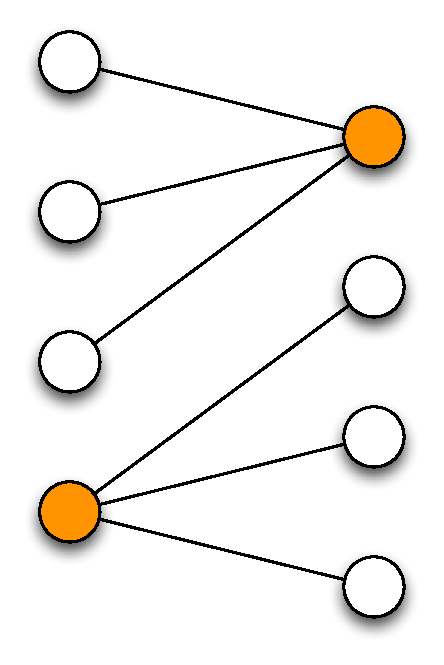
\includegraphics[width=\linewidth/3]{images/connection_graph.eps} \caption{Example of a bipartite connection graph with two concentrators of degree 3 marked as orange} 
	\label{fig:bipartite_graph} 
\end{figure}

In consequence of the fact that \emph{server sockets} provide a network application or service, they are likely to be contacted by several clients depending on their popularity. To this end, a socket which is contacted by a certain amount of client sockets and thus have a high degree in the connection graph is defined to be a \textbf{concentrator}. These concentrators are likely to offer a network service and are thus \emph{server sockets}. 
This approach is able to detect \emph{server sockets} which are offering not only classical client-server services,such as web, FTP, SSH, etc., but also p2p applications such as Skype, Bit-torrent super-nodes, etc. 
Therefore, it can be assumed that nodes with a high degree correspond to a \emph{server sockets}.

% introduce minimal vertex cover problem
\todo{Introduce Minimal vertex cover problem + recall + greedy algorithm}

% greedy algorithm to solve mvcp
% recalling sockets for optimization
\todo{Describe me!}
\begin{algorithm}[t!]
\caption{Detection of server sockets by \citet{Schatzmann:Mining,Schatzmann:Dissection, Schatzmann:Tracing}}
\label{alg:service_tracing_ss-detection}
\begin{algorithmic}
\STATE
\STATE compute list $SS_{in}$ \COMMENT{int. sockets sorted by \# ext. clients}
\STATE compute list $SS_{out}$ \COMMENT{ext. sockets sorted by \# int. clients}
\STATE
\WHILE{(deg($SS_{out}[0]$) $ > 2 $ \OR deg($SS_{in}[0]$)$ > 2$)}
    \WHILE {(deg($SS_{in}[0]$) $ > $ deg($SS_{out}[0]$))}
        \STATE $ss$ = $SS_{in}[0]$ \COMMENT{classify $ss$ as internal server socket}
        \STATE remove $ss$ from $SS_{in}$
        \STATE update deg() for all entries of $SS_{in}$
    \ENDWHILE
    \WHILE{(deg($SS_{out}[0]$) $ \geq $ deg($SS_{in}[0]$))}
        \STATE $ss$ = $SS_{out}[0]$ \COMMENT{classify $ss$ as external server socket}
        \STATE remove $ss$ from $SS_{out}$
        \STATE update deg() for all entries of $SS_{out}$
    \ENDWHILE
\ENDWHILE
\end{algorithmic}
\end{algorithm}

\begin{figure}
	[ht] \centering
	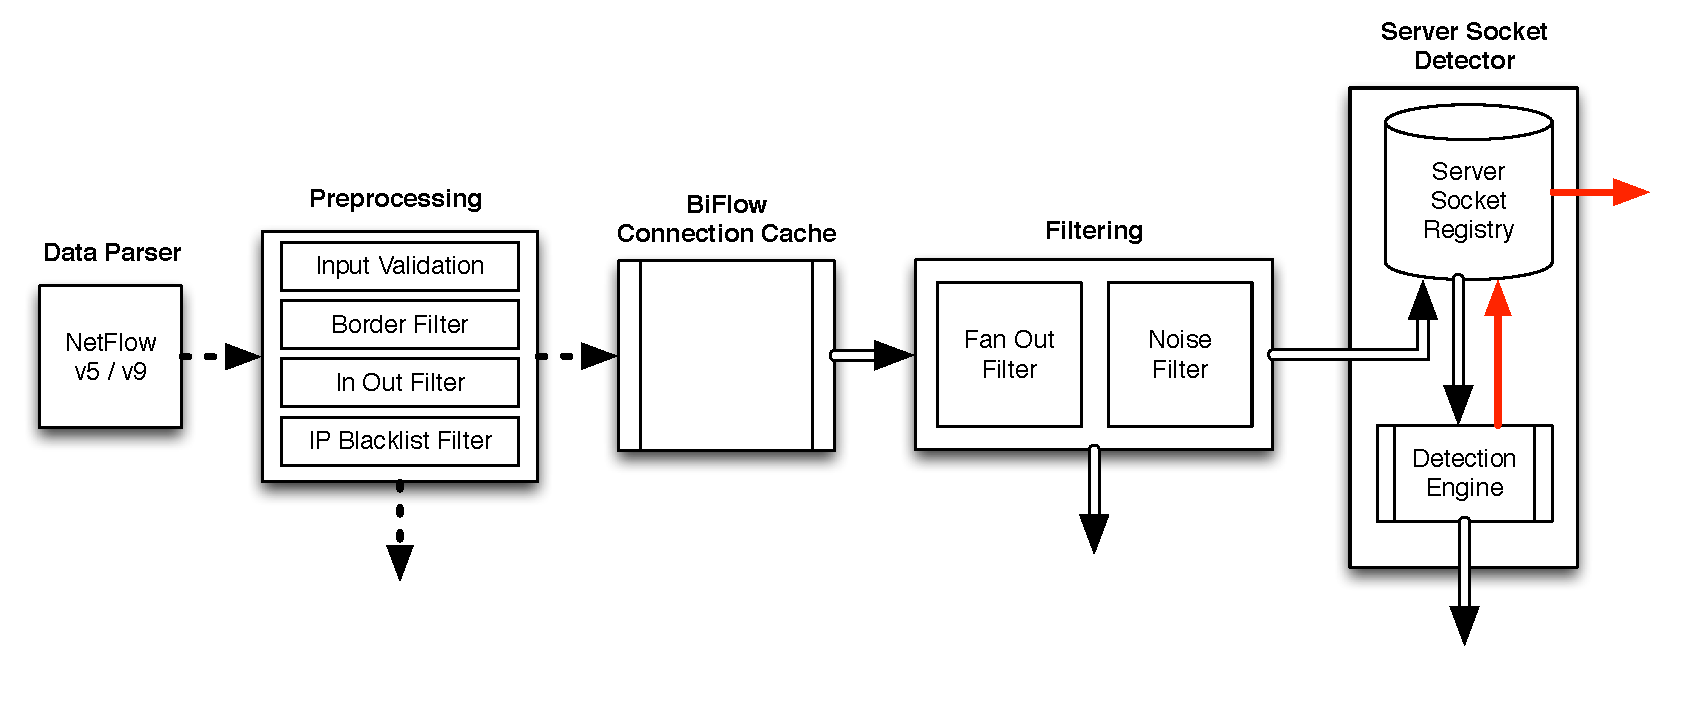
\includegraphics[width=\linewidth]{images/Detection_chain.eps}
	\caption{Processing chain for server socket detection} 
	\label{fig:detection_chain} 
\end{figure}

\subsection{Implementation}
Figure \ref{fig:detection_chain} illustrates the processing steps of the 
overall detection chain. The data parser is responsible to read the netflow data 
either in NetFlow v5 or NetFlow v9 format. These unidirectional flow records are 
then preprocessed by different blocks. While the input validator is performing 
some basic sanity checks of the flow data, the preprocessing filters are 
limiting the number of flows to the required kind of flow data. On the one hand, 
the border filter is removing all flow records not generated by a border router 
interface to efficiently prevent duplicate flow records. On the other hand, the 
In-Out filter is removing all non cross-border traffic, i.e. transit traffic 
(external to external) or entirely internal traffic (internal to internal). 
Furthermore, the IP blacklist filter is removing traffic towards blacklisted IP 
addresses or networks.

The connection cache is responsible for summarizing all related unidirectional 
flow records into a single bidirectional flow record during an aggregation 
period. After this caching step, these bidirectional flows are filtered by a fan 
out filter implementing the idea of \citet{Allman:2007} to mitigate the effects 
of scanning and p2p churn. This scanning detection filter is discussed in more 
detail by \citet{Schatzmann:Mining,Schatzmann:Dissection, Schatzmann:Tracing}. 

Afterwards, the remaining bidirectional flow records are again reduced by the 
noise filter. This last filtering module is responsible to filter bidirectional 
flow records which does not represent a correct bidirectional connection. A 
correct bidirectional connection is simply defined as either a correct TCP 
handshake or a reply flow as in case of UDP. Hence, the approach of deducing 
correct connections is to investigate the number of packets for each direction 
of the bidirectional flow record, i.e. the outgoing and the incoming flow 
record, since there are only cross-border flows remaining due to the In-Out 
filter. If a bidirectional TCP flow has in a single direction less than 3 
packets, the filter assumes that this flow does not represent a correct 
connection and is filtering this record. Accordingly, a bidirectional UDP 
flow is required to consist of at least 1 packet for each unidirectional flow 
record.

After these filtering steps, the remaining bidirectional flows are passed to the 
server socket detector which is finally performing the server socket detection 
approach previously discussed. Mainly, the server socket detector is build from 
two main parts. On the one side, there is the server socket registry which is 
containing all already known server sockets. On the other side, the detection 
engine implements the server socket detection algorithm. 

Firstly, the sockets of all bidirectional flows are queried against the current 
server socket registry if they are already known. If this is the case, the 
corresponding bidirectional flow records are removed and only the remaining flow 
records are passed to the detection engine to increase the efficiency of the 
detection algorithm. The detection engine is building the bipartite connection 
graph and is detecting the concentrators of it. These detected server sockets 
are then passed to the server socket registry so that these sockets may be 
recalled afterwards. 

Finally, the server socket registry is able to output all detected server 
sockets of the observation period. 

%%%%%%%%%%%%%%%%%%%%%%%%%%%%%%%%%%%%%%%%%%%%%%%%%%%%%%%%%%%%%%%%%%%%%%%%%%%%%%%%
% MONITORING OF SERVER SOCKETS
%%%%%%%%%%%%%%%%%%%%%%%%%%%%%%%%%%%%%%%%%%%%%%%%%%%%%%%%%%%%%%%%%%%%%%%%%%%%%%%%
\newpage
\section{Monitoring of Server Sockets 
\label{section:socket_tracking}}

The previous section outlined the approach of detecting \emph{server sockets}. 
This section covers the approach of monitoring flow data and generating 
statistical information such that some characteristics and properties of the 
found \emph{server sockets} can be assessed as outlined in section 
\ref{section:characterization}.

\subsection{Server Socket Statistics}

The monitoring of the external 
\emph{server sockets} is done with help of the \emph{server socket registry} 
which is already used in the detection approach. This registry recalls all 
\emph{server sockets} which are known yet. 

Hence, all flows originated from a \emph{server socket} or flows which are 
destined for a \emph{server sockets} are monitored for compiling the socket 
statistics later used for the characterization.

In contrast to the detection approach, there are no scanning or other noise 
filters in the processing chain, because of the fact that they will remove at 
least some flows, mainly unidirectional flows, which are actually relevant for 
the statistics. 

Since the processing is based on data containing flows which are active within a 
certain time slot, the statistics are accounted on a the same discrete time 
scale, i.e. 10 minutes. 

At first, each flow is checked if it is a flow of a \emph{server socket}. If 
this is the case, the individual flow statistics are accounted to the 
corresponding specific server socket \textbf{statistics record}. This includes 
the following entries: 

\vbox{
\begin{itemize}
	\item Number of bidirectional connections 
	\item Number of outgoing unidirectional connections 
	\item Number of incoming unidirectional connections 
\end{itemize}
}

In second step, the statistics records of each discrete time slot are aggregated in such a way that the information of the activity within a certain time slot is kept. Thus, the overall server socket statistics record contains the following entries: 

\vbox{
\begin{itemize}
	\item Sum of bidirectional connections of each time slot 
	\item Sum of outgoing unidirectional connections of each time slot 
	\item Sum of incoming unidirectional connections of each time slot 
	\item Number of days with connections 
	\item Number of discrete time slots with connections 
	\item Timestamps of discrete time slots with connections 
\end{itemize}
}

\subsection{Traffic Statistics} 

Besides of the individual server socket statistics report, overall traffic statistics are accounted, mainly for deducing knowledge of how good the monitoring capability of the server sockets in the registry is. For this reason, each flow which belongs to a server socket which is present in the registry is denoted as monitored. Hence, flows which does not belong to a server socket are accounted as not monitored. 

Moreover, all unmonitored flows can be further investigated for better understanding of the type of this unmonitored traffic. This can be done on the following three scopes: 
\begin{itemize}
	\item Protocol level 
	\item Port level for UDP and TCP flows 
	\item Location of the connection end-points 
\end{itemize}

The first scope captures statistical information of the problem that server sockets are only defined for protocol TCP and UDP, hence all flows with another protocol are per definition unmonitored.

Secondly, there are statistics generated for all unmonitored TCP or UDP flows which don't have a corresponding server socket in the registry present. There are various reasons for this, mainly related to the detection approach outlined in section \ref{section:socket_detection}. In most of the cases, the sockets are not contacted by enough clients, therefore, the are not detected as concentrators and in consequence of that not denoted as server sockets. Furthermore, scanning activity is also a major contributor to this unmonitored flows, since scanning traffic and other non-legitimate traffic is removed before the server socket detection is performed. Consequently, these scanned sockets are not detected as server sockets, in case there is no legitimate traffic towards these sockets.

On the one hand, there is the possibility to account for each port the unmonitored flows which will lead to very detailed statistical information about the missed server sockets. However, this comes at the price of an inefficient processing and higher memory usage. 

On the other hand, the flows can be categorized by port ranges. In this thesis, there are just two ranges defined for this categorization:

\begin{itemize}
	\item Low port: 0-1023 
	\item High port: 1024-65365 
\end{itemize}

These categories are further divided by the location of the socket either internal or external and thus involving the third scope. Hence, the unmonitored TCP and UDP flows or strictly speaking the corresponding sockets are accounted by the following four categories:

\vbox{
\begin{itemize}
	\item external port high, internal port high 
	\item external port high, internal port low 
	\item external port low, internal port high 
	\item external port low, internal port low 
\end{itemize}
}

All these general traffic statistics allows to deduce insights about the properties of the detection process by learning what is missed. Moreover, these general traffic statistics are revealing information about the properties of the current server socket set with respect to traffic representation and thus about some properties of this set. 

\subsection{Implementation}

Figure \ref{fig:monitoring_chain} shows the modular implementation of the 
server socket monitoring chain. Comparing the monitoring chain to the detection 
chain from figure \ref{fig:detection_chain} it is clearly visible that the 
modules up to the bidirectional connection cache are shared. However, in the 
monitoring chain there are no fan-out filter and noise filter applied. This is 
because every traffic destined to a server socket should be considered, 
therefore no bidirectional flow records are filtered before accounting them. The 
server socket monitor is accounting the general traffic statistics as well as 
the individual server socket statistics.

First of all, the bidirectional flow records are separated into those belonging 
to a known server socket, denoted as monitored traffic, and those not belonging 
known server socket, denoted as unmonitored traffic. To be more precisely, this 
is done by querying the server socket registry which is loaded with previously 
detected server sockets. Then, the traffic monitor investigates the monitored 
and unmonitored traffic for generate the overall traffic statistics. 
Furthermore, it examines the unmonitored traffic even more closely for deducing 
the knowledge about the other traffic statistic scopes as protocol, direction 
ports and type of connection.\todo{Correct?!}

\begin{figure}[hb]
	\centering
	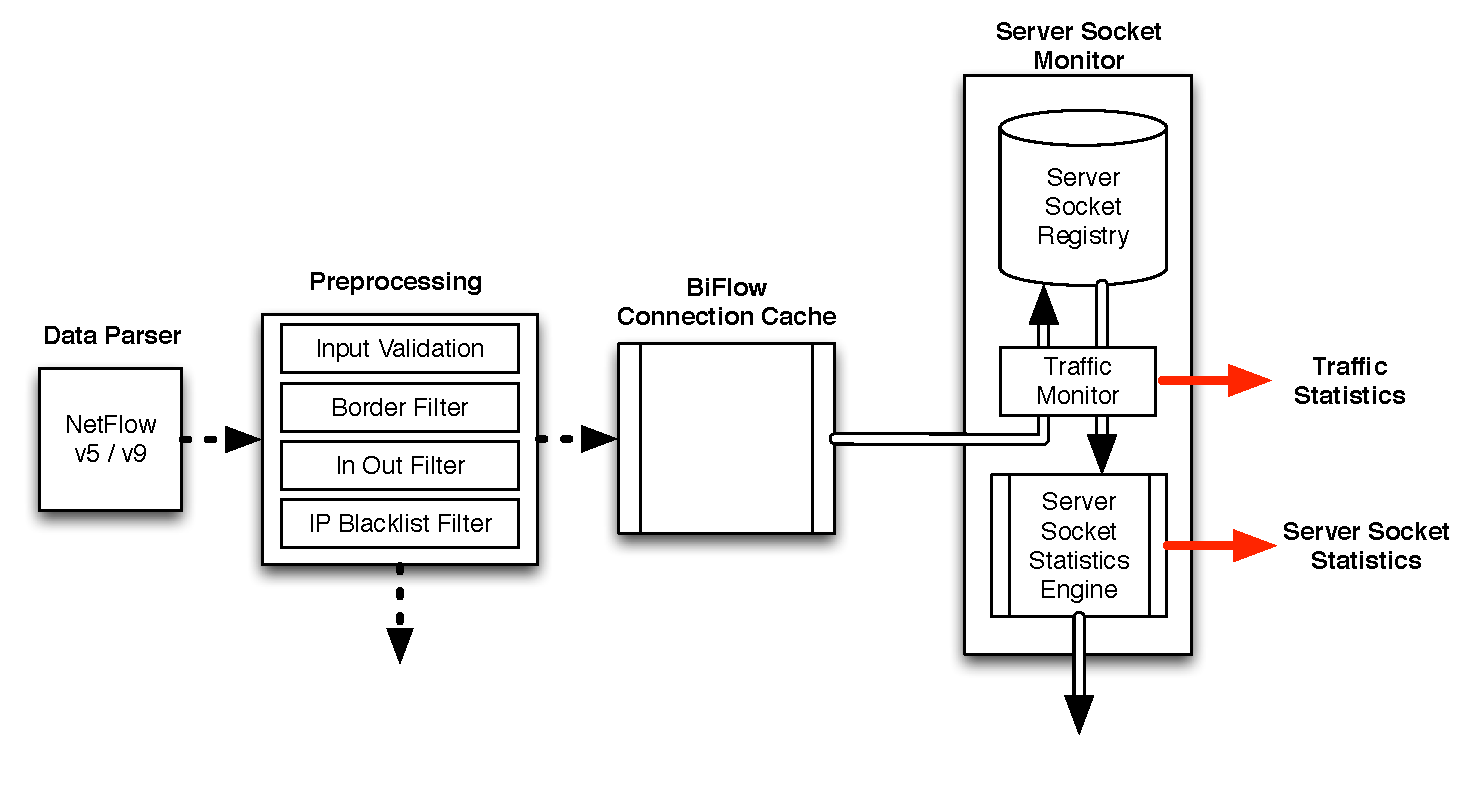
\includegraphics[width=\linewidth]{images/TrackingChain.eps}
	\caption{Processing chain for the server socket monitoring} 
	\label{fig:monitoring_chain} 
\end{figure}

%%%%%%%%%%%%%%%%%%%%%%%%%%%%%%%%%%%%%%%%%%%%%%%%%%%%%%%%%%%%%%%%%%%%%%%%%%%%%%%%
% CHARACTERIZATION SERVERSOCKETS
%%%%%%%%%%%%%%%%%%%%%%%%%%%%%%%%%%%%%%%%%%%%%%%%%%%%%%%%%%%%%%%%%%%%%%%%%%%%%%%%
\newpage
\section{Characterization of Server Sockets 
\label{section:characterization}} The main interest of this thesis is to characterize \emph{server sockets} by its \textbf{stability}, its \textbf{visibility} and its \textbf{popularity}. These properties tries to address the following characteristics of a server socket:

\vbox{ 
\begin{itemize}
	\item \textbf{Stability:} How stable is the \emph{server socket} regarding its responsiveness or availability: 
	\item \textbf{Visibility:} How frequently is the \emph{server socket} contacted by other socket: 
	\item \textbf{Popularity:} How many distinct sockets are contacting the \emph{server socket}: 
\end{itemize}
}

These three characteristics are directly deducible from the statistics observed by the passive monitoring technique outlined in \ref{section:socket_tracking}. In the following, each of the three characteristics are briefly discussed.

\subsection{Stability of a Server Socket} Because of the definition and its detection approach a \emph{server socket} is offering a bidirectional service which means that the client and the \emph{server socket} are both sending packets. Usually, a client socket is opening the connection to a \emph{server socket} which will reply in return to this request. Generally, this also holds for P2P applications as for example bit torrent. However in this case, there may be two \emph{server sockets} involved in the communication and no client socket. Therefore, a \emph{server socket} -- or the communication of it -- can be characterized as stable if all connections of this \emph{server socket} are \textbf{balanced}. 

%%%%%%%%%%% Balanced Connection DEFINITION 	%%%%%%%%%%%%%%%%%%%%%%
\parbox{ 
\textwidth}{ 
\begin{defn}
	{\textbf{Balanced Connection}\\} A connection between two sockets is balanced, if there is one flow originating from each socket which is destined for the other socket. Hence, the connection is bidirectional. 
\end{defn}
}

Thus, the overall stability \emph{server socket} or availability of its service can be approximated by the ratio of the balanced to all connections destined to this \emph{server socket}, i.e. the balanced and the unbalanced. This ratio is referred as a \emph{server socket} \textbf{stability ratio} and is mathematically defined by equation \ref{eq:ratio}. 
\begin{equation}
	\text{Stability}(\text{Socket}_i) = \frac{\text{balanced connections}(\text{Socket}_i)}{\text{balanced connections}(\text{Socket}_i) + \text{unbalanced connections}_{in}(\text{Socket}_i)} 
	\label{eq:ratio} 
\end{equation}

Hence, a \emph{server socket} with a stability ratio of 1 does only have bidirectional connections and thus, replies to all connection attempts. On the other side, a stability ratio of 0 indicates that there are only connections attempts by client sockets, but the server socket never replied upon these request. Unbalanced outgoing connections from the server sockets are indicating a client error or scanning activities of clients with spoofed (internal) source address which are not observed by the monitoring system. Therefore, these unbalanced outgoing connections are not considered for determining the stability ratio at all.

\subsection{Visibility of a Server Socket\label{subsection:visibility}}

% discrete time slots activities of a socket, per day, per 5min slot?
% distribution is heavy-tailed, alot of sockets only rarely connected => due to scanning? due to malware?
The monitoring process of the server sockets is done passively, thus if a server socket is visible in the flow level data of a certain time period, the server socket is active during at that time. Hence, the visibility of a server socket during a certain time interval $t+\Delta{t}$ is a binary measure, either inactive in case it is not visible or active in case it is visible in the data set. Equation \ref{eq:visibility} defines the visibility of a socket during the time interval $t+\Delta{t}$: 
\begin{equation}
	\text{Visibility}_t(\text{Socket}_i,t+\Delta{t}) = \left\{ 
	\begin{array}{l l}
		1 & \quad \text{if $\text{Socket}_i$ is active during $t+\Delta{t}$}\\
		0 & \quad \text{if $\text{Socket}_i$ is not active during $t+\Delta{t}$}\\
	\end{array}
	\right. 
	\label{eq:visibility} 
\end{equation}

In consequence, there are different granularities $\Delta{t}$ to define the visibility a server socket. On the one hand, the most fine-grained resolution is just the flow-level data observation period. In most of the cases, this flow-level data observation period is set to 300 seconds. This fine-grained resolution is referred as the \emph{time slot} resolution, since the entire processing is based on such discrete time slotted data, containing all flows active during this time period. 
On the other hand, there are several other more coarse-grained resolutions of the visibility possible. The most obvious is a day long resolution, i.e. $\Delta{t} = 86400$s.

Furthermore, the visibility of a server socket can be extended from a single time period to the overall observation time, i.e. a week long trace, by summing up the individual visibilities of each time slot as shown in equation \ref{eq:visibility_sum}.
\begin{equation}
	\text{Visibility}(\text{Socket}_i) = \sum_{t} \text{Visibility}_t(\text{Socket}_i,t+\Delta{t})
	\label{eq:visibility_sum} 
\end{equation}

However, this summing approach exacerbate the comparison between different observations since it represents the visibility in absolute terms. Therefore, an even better metric for the visibility of a server socket is to average the individual $\text{Visibility}_t(\text{Socket}_i,t+\Delta{t})$ as outlined by equation \ref{eq:visibility_avg}. This normalizes the visibility to a value in the range between 0 and 1, representing the ratio of its visibility to the maximum visibility possible. Thus, a value of 1 means that the socket is visible in every single time slot and a value of 0 that the socket was never active. 
\begin{equation}
	\overline{\text{Visibility}}(\text{Socket}_i) = \frac{\sum_{t} \text{Visibility}_t(\text{Socket}_i,t+\Delta{t})}{\sum_{t}1}
	\label{eq:visibility_avg} 
\end{equation}

\subsection{Popularity of a Server Socket}

% number of flows / clients?.. degree of Server Socket
Besides the visibility of a server socket, its popularity is another major key characteristics. Whereas the visibility of a server socket defines how frequent in time a socket is contacted by at least one connection endpoint, the popularity of a server socket is defined by the number of connection attempts of client sockets during a certain period of time. The popularity of server socket can be deduced by various metrics as the number of flows, bytes or clients.


%%%%%%%%%%%%%%%%%%%%%%%%%%%%%%%%%%%%%%%%%%%%%%%%%%%%%%%%%%%%%%%%%%%%%%%%%%%%%%%%
% ANALYSIS of SERVER SOCKETS IN THE WILD
%%%%%%%%%%%%%%%%%%%%%%%%%%%%%%%%%%%%%%%%%%%%%%%%%%%%%%%%%%%%%%%%%%%%%%%%%%%%%%%%\newpage
\section{Analysis of Server Sockets in the Wild}

This section covers a detailed analysis of server socket found during a week long data trace from 2010/11/01 00:00:00 UTC until 2010/11/06 00:49:00 UTC, thus covering mainly the first 5 working days in November 2010.

\subsection{Detected Server Sockets}

% sum up of detection parameters > 2 biflows per 5min interval with more TCP 
% packets > 3 UDP > 1
For detecting the server sockets in this observation period, the previously 
discussed detection approach was applied as illustrated by figure 
\ref{fig:detection_chain}. In detail, the connection cache was configured to 
summarize all related unidirectional flow records into a single bidirectional 
flow record during an aggregation interval of 600s. 

After this caching step, these bidirectional flows are filtered by a fan out 
filter implementing the idea of \citet{Allman:2007} to mitigate the effects of 
scanning and p2p churn. This fan out filter is configured to require at least 4 
unidirectional connections with a certain host as source and at least 2 times 
more unidirectional connections than bidirectional connections for classifying 
this host as a scanning host. Previous 
work\citep{Schatzmann:Mining,Schatzmann:Dissection, Schatzmann:Tracing} has 
shown that these parameters are a good choice for efficiently mitigating the 
scanning noise by reducing the scanning spikes of the total traffic volume. 

Moreover, the noise filter is configured to filter all TCP flows with less than 
3 packets in a single direction and UDP flows with less than 1 packet in a 
single direction. 

Furthermore, the server socket detector is configured to extract sockets with a 
degree of 2 or higher as concentrators, thus defining requiring two independent 
connections to a server sockets within 600 seconds. 

% state overall number of detected external and internal server sockets during 
% this period
During the entire observation period of 120.8 hours, the server socket detector 
managed to detect 1'862'389 external server sockets and 609'670 internal server 
sockets.

\subsection{Gravitational Forces of Server Sockets}
% traffic statistics of server sockets detected by type and ratio of traffic 
% towards server sockets
In the following, the overall traffic statistics of the detected server sockets 
are briefly discussed. Figure \ref{fig:flows_by_type} shows the absolute number 
of flows during the entire observation period separated by the type of 
connection. If the flow is destined to a server socket, the flow is denoted as 
monitored, otherwise if as unmonitored. Furthermore, the type of connection also 
considers the balance or direction of the connection, i.e. if the flow is 
bidirectional, unidirectional outgoing or unidirectional incoming. Hence, in 
total there are 6 possible combinations for the type of connection, allowing a 
good interpretation of the detection approach. For easier comparison of each 
type of connection, figure \ref{fig:monitored_flows_by_type} shows the ratio of 
monitored and unmonitored flows by the direction.

In figures \ref{fig:flows_by_type} and \ref{fig:monitored_flows_by_type}, there are two gaps visible around 2010/11/01 10:00 UTC and 2010/11/04 06:05 UTC. These gaps result from missing flow records due to router reboots, collector outages, and storage failures\citep{Schatzmann:Mining}.

\begin{figure}
	[ht] \centering 
	\includegraphics[width=\linewidth]{images/Flows_by_type_area_all_SeS.pdf}
	\caption{Number of flows over time by the type of connection with all detected server sockets} 
	\label{fig:flows_by_type} 
\end{figure}

\begin{figure}[h]
	\centering 
	\includegraphics[width=\linewidth]{images/Flows_monitor_ratio_by_type_all_SeS.pdf}
	\caption{Flows towards known server sockets by traffic type with all detected server sockets} 
	\label{fig:monitored_flows_by_type} 
\end{figure}

Clearly, the dominating kind of the flows are the bidirectional monitored flows 
represented by the red area in figure \ref{fig:flows_by_type}. Comparing this 
share with the bidirectional unmonitored flows represented by the yellow area 
between the red and the green area, yields that the detection approach detects a 
majority of the server sockets. This finding is even better visible on the 
bidirectional ratio of figure \ref{fig:monitored_flows_by_type}. Depending on 
the time of the day, the monitoring ratio of the bidirectional flows is mainly 
between 90\% and 97\%. There are always smaller monitoring ratios during night 
yielding that at night there is a higher share of unknown server sockets active 
than during day. A possible reason for pattern is that there are some server 
sockets which are regularly contacted, however only by very few clients so that 
these sockets get never more than one connection within 600 seconds. Thus, these 
sockets are never detected as concentrators. 

Similarly, if the unidirectional outgoing flows are examined by looking at figure \ref{fig:monitored_flows_by_type}, the monitored flows have predominantly a high share of around 80\% to 90\% of all unidirectional outgoing flows. Figure \ref{fig:flows_by_type} also reveals some high peaks which are probably scanning or backscatter effects which are well visible at November 03 in the night and in the afternoon by the green spikes. However, these green peaks are categorized as monitored unidirectional outgoing flows, thus they must involve at least one known server socket either located external or internal.

Finally, the unidirectional incoming flows have are predominately unmonitored with around 80-97\% of unmonitored flows as it can be seen in figure \ref{fig:monitored_flows_by_type}. Contrasting the trend of the other two categories of traffic, the main reason for this contrast may be that the main part of this unidirectional incoming traffic consists of Internet background radiation \citep{Wustrow10,Pang04} as for example malware scanning. Nevertheless, this unidirectional incoming flow traffic is unimportant with respect to the scope of this thesis.

In a metaphorical sense, server sockets are comparable to masses in physics which are exerting gravitational forces to other objects. Server sockets tend to attract a majority of the observed connections and thus, they are well suitable to represent a majority of the legitimate traffic which is interesting for tracking the end-to-end connectivity.

\todo{Comparing with Port80 SES?!}

\newpage
\subsection{Characterization of Detected Server Sockets}

As discussed in section \ref{section:characterization}, this thesis proposes to characterize server sockets according to their visibility, popularity and stability by different metrics. This section aims to deduce some statistical properties of the detected server sockets regarding these characteristics.

\subsubsection{General Visibility of Server Sockets}

According to \ref{subsection:visibility}, for defining a metric of the visibility of server sockets it is required to define the granularity of a observation period. For reasons of simplicity, two different granularities are defined. One the one hand, a day long observation period yields the number of visible days for the activity of a socket. On the other hand, an observation period of 5 minutes is chosen, since it reflects the default processing interval of FlowBox, allowing a very fine-grained, detailed resolution of a server sockets activity. This second visibility metric is referred as \emph{visible time slots(VTS)}.

\begin{figure}
	[hb] \centering 
	\includegraphics[width=\linewidth]{images/VTS_by_visibledays.pdf}
	\caption{VTS by visible days} 
	\label{fig:vts_by_visibledays} 
\end{figure}

Figure \ref{fig:vts_by_visibledays} shows the number of sockets by the visible time slots separated the number of visible days. The skewness of the 
distributions for 1 to 4 visible days are is very similar. It is obvious that 
the a socket which is visible for only one day cannot exceed 288 visible time 
slot. Nonetheless, considering this daily scaling factor, the distributions are 
looking very similar. Furthermore, figure \ref{fig:vts_by_visibledays} shows 
that the most sockets in absolute terms are only active during one day and only 
in very few visible time slots. 

However, the distribution of the number of sockets with a visibility of 5 or 
even 6 days are slightly different, since there is a higher share of sockets 
with a relatively higher visible time slots, besides the normal scaling factor 
of the number of visible days.

\subsubsection{Visibility and Stability}
Eventually, for selecting those server sockets which are stable and often visible it is of importance to assess the how server sockets are distributed with respect to their stability and visibility characteristic. Hence, figure \ref{fig:rankedVisibility} shows the location of each socket in the field of the ranked visibility and the stability. The ranked visibility is simply defined by the cumulative distribution function of the visibility. Thus, a socket with a ranked visibility of 80\% indicates that there are 80\% of all sockets with the same or lower visibility than this specific socket. 

As figure \ref{fig:rankedVisibility} indicates, the sockets cluster around the top right corner, hence the top visible sockets tend to have a good stability as well.

\begin{figure}
	[hb] \centering 
	\includegraphics[width=\linewidth]{images/visibiliy_stability_map.pdf}
	\caption{Sockets by their ranked visibility and their stability} 
	\label{fig:rankedVisibility} 
\end{figure}


Furthermore, figures \ref{fig:ccdf_ratio_days} and \ref{fig:ccdf_ratio_vts} show 
each a complementary cumulated distribution function of the stability of server 
sockets with different visibilities. 

One the one side, figure \ref{fig:ccdf_ratio_days} is using the daily visibility 
of the sockets. The red curve represents the distribution of the sockets which 
are seen only in one day. Not surprisingly, these group of server sockets reveal 
the highest share of sockets with a stability of 1. This is mainly due to the 
fact that there is a relative high number of server sockets with which are 
active only during a relatively short period of time. This can be justified by 
looking at figure \ref{fig:vts_by_visibledays}.



\begin{landscape}
\begin{figure}
	[p] \centering 
	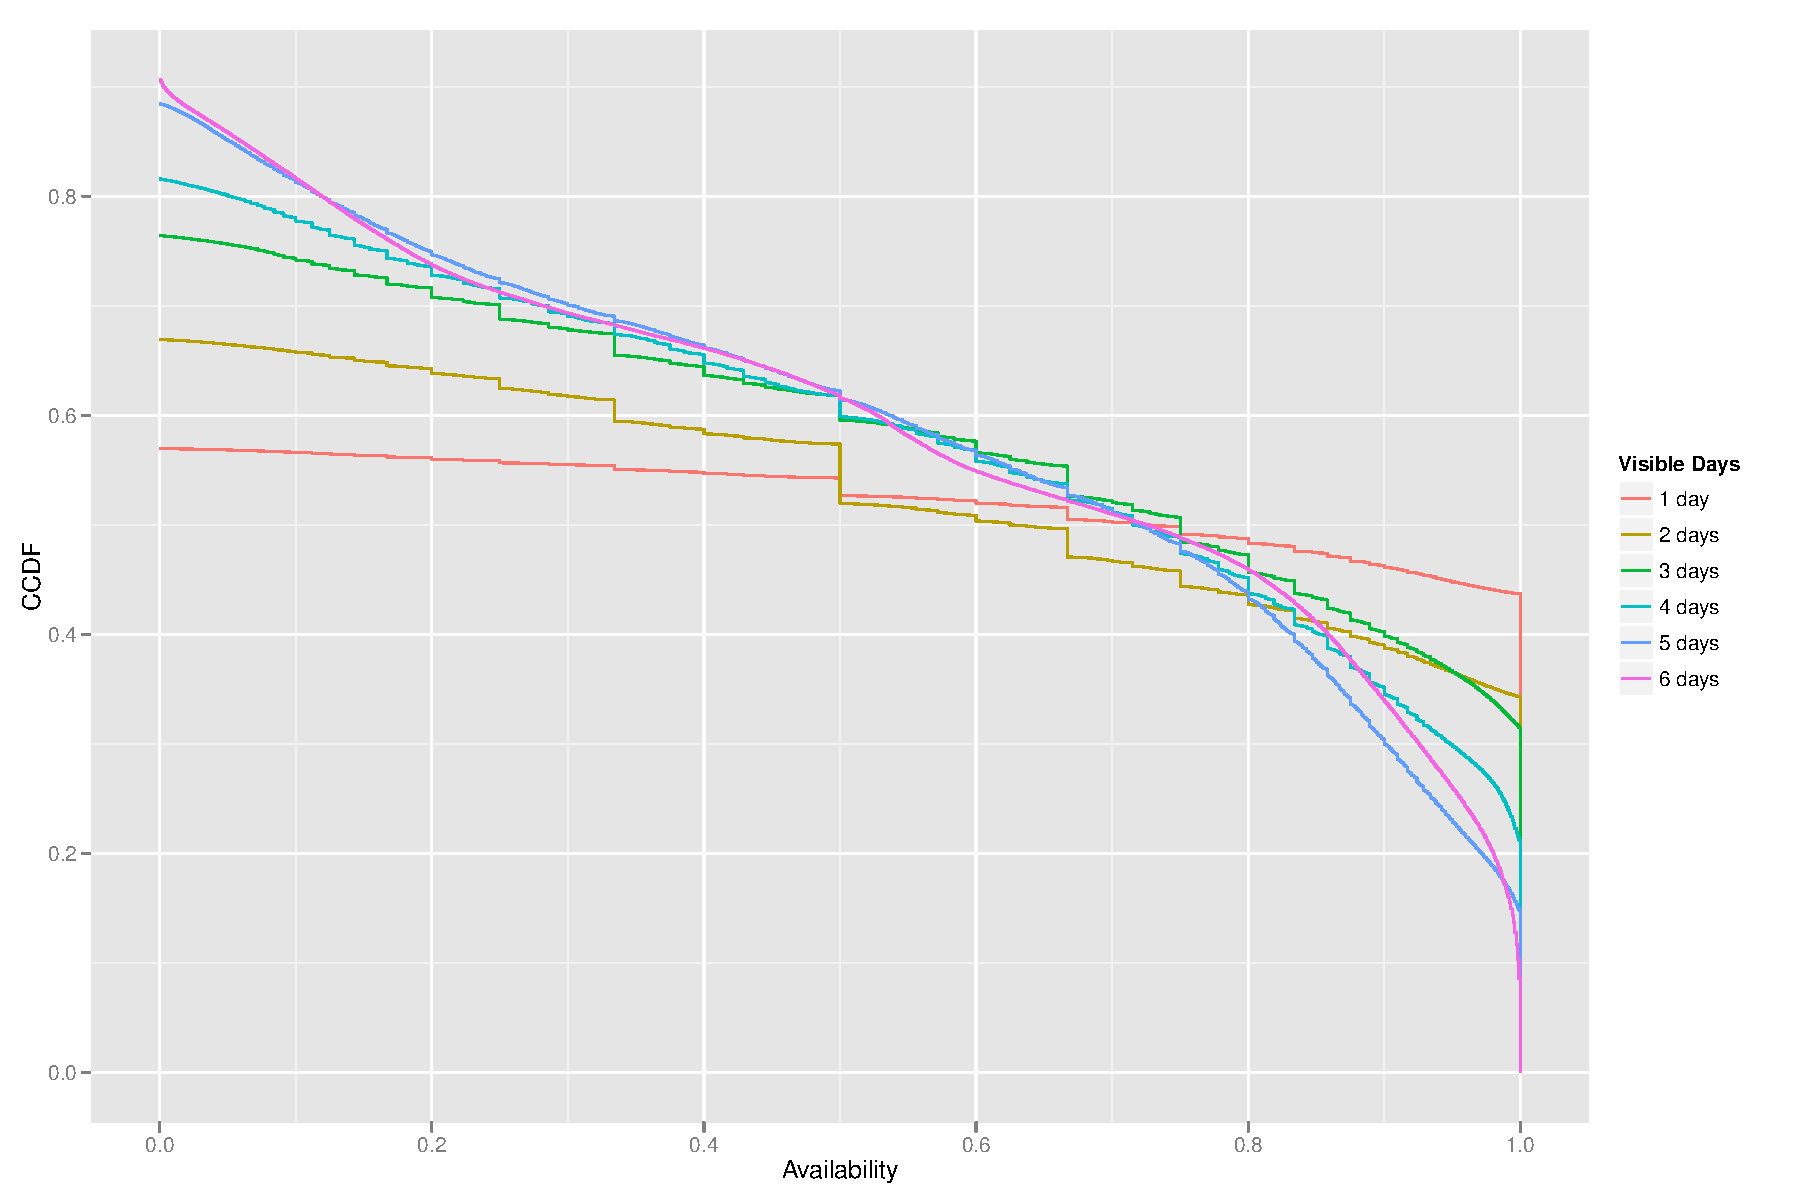
\includegraphics[width=\linewidth]{images/CCDF_ratio_days.pdf}
	\caption{CCDF of the availability by visible days} 
	\label{fig:ccdf_ratio_days} 
\end{figure}
\end{landscape}

\begin{landscape}
\begin{figure}
	[p] \centering 
	\includegraphics[width=\linewidth]{images/CCDF_ratio_VTS.pdf}
	\caption{CCDF of the availability by visible time slots} 
	\label{fig:ccdf_ratio_vts} 
\end{figure}
\end{landscape}

\subsubsection{Popularity and Stability}
Similarly to the visibility, the server sockets characteristics of popularity 
and stability are briefly assessed in the following. The ranked popularity is 
defined in the same way as the ranked visibility. To be precise, the ranked 
popularity is defined as the cumulative distribution function of the popularity 
in terms of flows. Hence, a server socket with a ranked popularity of 80\% 
signifies that there are 80\% of all server socket with a lower or equal 
popularity as this specific socket.


\begin{figure}
	[ht] \centering 
	\includegraphics[width=\linewidth]{images/popularity_stability_map.pdf}
	\caption{Sockets by their ranked popularity and their stability} 
	\label{fig:rankedPopularity} 
\end{figure}


\begin{landscape}
	\begin{figure}
	[p] \centering 
	\includegraphics[width=\linewidth]{images/top20_ratio_box.pdf}
	\caption{Boxer plot of the availability / stability of the top 20 traffic port server sockets} 
	\label{fig:top20_ratio_box} 
\end{figure}
\end{landscape}

\begin{landscape}
\begin{figure}
	[p] \centering 
	\includegraphics[width=\linewidth]{images/top20_visibility_box.pdf}
	\caption{Boxer plot of visibility in days of the top 20 traffic port server sockets}
	\label{fig:top20_visibledays_box}
\end{figure}
\end{landscape}


\begin{table}
	[ht] \centering 
	\begin{tabular}
		{|c|r|r|r|r|r|r|} \hline \textbf{Position} & \textbf{Port} & \textbf{Protocol} & \textbf{Flows} &\textbf{ Flows in \%} & \textbf{Sockets} & \textbf{Sockets in \%}\\
		\hline \hline 1 & 53 & 17 &793851107 & 47.272216 & 314253 & 18.68397\\
		\hline 2 & 80 & 6 &623910956 & 37.152626 & 546735 & 32.50623\\
		\hline 3 & 443 & 6 & 74333936 & 4.426434 & 59800 & 3.555420\\
		\hline 4 & 22 & 6 & 10580812 & 0.630066 & 40363 & 2.399790\\
		\hline 5 & 2703 & 6 & 10139578 & 0.603791 & 22 & 0.001308\\
		\hline 6 & 25 & 6 & 6943533 & 0.413473 & 18560 & 1.103488\\
		\hline 7 & 123 & 17 & 4988781 & 0.297072 & 286 & 0.017004\\
		\hline 8 & 993 & 6 & 3844043 & 0.228905 & 1398 & 0.083118\\
		\hline 9 & 555 & 6 & 3290709 & 0.195955 & 9 & 0.000535\\
		\hline 10 & 995 & 6 & 2411245 & 0.143585 & 654 & 0.038884\\
		\hline 11 & 110 & 6 & 1816240 & 0.108153 & 1211 & 0.072000\\
		\hline 12 & 3789 & 6 & 1796224 & 0.106961 & 10 & 0.000595\\
		\hline 13 & 53 & 6 & 1726716 & 0.102822 & 1102 & 0.065520\\
		\hline 14 & 2128 & 6 & 1677027 & 0.099864 & 390 & 0.023188\\
		\hline 15 & 3478 & 17 & 1607132 & 0.095701 & 176 & 0.010464\\
		\hline 16 & 8080 & 6 & 1362615 & 0.081141 & 2056 & 0.122240\\
		\hline 17 & 3128 & 6 & 1298424 & 0.077319 & 191 & 0.011356\\
		\hline 18 & 5354 & 6 & 1221109 & 0.072715 & 3 & 0.000178\\
		\hline 19 & 8001 & 6 & 1014631 & 0.060419 & 58 & 0.003448\\
		\hline 20 & 21 & 6 & 1010771 & 0.060189 & 1419 & 0.084367\\
		\hline 21 & high & 6 & 37679906 & 2.243762 & 599314 & 35.63233\\
		\hline 22 & high & 17 & 89558306 & 5.333015 & 89820 & 5.340265\\
		\hline 23 & low & 6 & 2505504 & 0.149198 & 3807 & 0.226346\\
		\hline 24 & low & 17 & 749276 & 0.044618 & 302 & 0.017955\\
		\hline 
	\end{tabular}
	\caption{Top 20 port / protocol aggregated sockets by number flows}
	\label{tab:top20_ports}
\end{table}\todo{do something with me..}
SSH TCP 22: Scanning / PW guessing, e.g. X.X.X.X, 6, 22, 1.0, 2, 1, 69.0, 0.0, 0.0 always with 69 or 68 biflows (parallelized? recurring?) $\rightarrow$ that's way such a bad visibility! one-time shots.. /8 network is scanned! meist 3-4 timeslots und nur visibility einem Tag! \ref{tab:top20_ports}\todo{do something with me..}
 

mDNS (5354) $\rightarrow$ Apple mdns resolving; mainly one socket causing this traffic pm-members.apple.com

%!TEX root = ./main.tex
%** 50_integration.tex
\chapter{Extending FACT with Server Sockets\label{chapter:integration}}

\section{Smart Traffic Selection using Server Sockets Sets}


% outline that this is a optimization problem which is approximated by several socket sets however not guaranteed to be optimal



%!TEX root = ./main.tex
%** Results.tex: What were the results achieved including an evaluation
\chapter{Evaluation\label{chapter:results}}

In order to evaluate the effect of server socket based traffic preselection, three known events were analyzed with the old port-based heuristic of FACT as well as with the new server socket based approach. Then, both results are compared and the effect of the traffic preselection on the noise of the results is qualitatively discussed.

Table \ref{table:ses_set_coverage} shows the coverage of each set with respect to their IP space coverage in absolute and relative terms. 

% state the sets which are what coverage in terms of /24, IP SPACE v4/v6
\todo{FIXME!!}
\begin{table}
	[ht] \centering 
	\begin{tabular}
		{|l|c|r|r|r|r|} \hline \multirow{2}{*}{\textbf{Socket Set}} & \multirow{2}{*}{\textbf{Number of Sockets}} & \multicolumn{2}{|c|}{\textbf{IPv4 Space}} & \multicolumn{2}{|c|}{\textbf{IPv6 Space}} \\
		\cline{3-6} & & absolute & relative & absolute & relative \\
		\hline \hline All Server Sockets & 2129033 & 694627 & 100\% & 1231 & 100\% \\
		\hline Port 80 & 610273 & 158765 & 22.85\% & 296 & 24.05\% \\
		\hline Port 53 \& 80 & 939345 & 238032 & 34.27\% & 1153 & 93.66\% \\
		\hline Port 53 \& 80 \& 443 & 1010966 & 251044 & 36.14\% & 1157 & 93.99\% \\
		\hline 
	\end{tabular}
	\label{table:ses_set_coverage}
	\caption{Coverage of server socket sets} 
\end{table}

\todo{state that socket sets are from november 2010, events are before! due to lack of time to do detection for each event }


%%%%%%%%%%%%%%%%%%%%%%%%%%%%%%%%%%%%%%%%%%%%%%%%%%%%%%%%%%%%%%%%%%%%%%%%%%%%%%%%
% EVENT 1: AMS-IX PARTITIONING
%%%%%%%%%%%%%%%%%%%%%%%%%%%%%%%%%%%%%%%%%%%%%%%%%%%%%%%%%%%%%%%%%%%%%%%%%%%%%%%%
\section{Event 1: Partitioned Internet Exchange Point}

The IXP \citet{AMS-IX}(AMS-IX) performed on March 23, 2010 a scheduled maintenance. When its connection to \citet{switch} came back, there was only a partial connectivity through this IXP, since some next-hops learned via their route servers were not properly reachable, thus traffic towards these networks are black-holed.\citep{SchatzmannPAM2011}

In consequence, several internal clients of the \citet{switch} network were complaining about unreachable external services on the next morning. Using classical debugging tools, it took more than four hours for fixing the problem by resetting a port.\citep{SchatzmannPAM2011}

\subsection{Heuristic Approach}
This event is well visible by the classical FACT, since there are quite a large number of affected users thus favoring the user aggregation approach of detecting relevant events. Figure \ref{fig:AMS_IX_FACT_REF} shows the number of unreachable BGP prefixes over time separated by the number of affected internal clients. As previously outlined the user aggregation approach tries to prioritize severe events by determining the number of affected internal users. Hence, the severity of the events is indicated by the color of the unreachable prefixes in figure \ref{fig:AMS_IX_FACT_REF}. To be precise, the pink prefixes denotes the unreachable prefixes by at least 10 distinct internal clients, the blue respectively 5 distinct internal clients.

This specific IXP partitioning event is clearly visible in figure  \ref{fig:AMS_IX_FACT_REF} from 05.00 UTC to 08:15 UTC with almost 20 unreachable BGP prefixes affecting more than 10 internal clients and almost 200 unreachable BGP prefixes in total. However, as discussed in chapter \ref{Introduction}, those unreachable prefixes affecting only 1 client are not reliable observations, thus of limited interest representing a kind of observation noise of FACT.

\begin{figure}
	[p] \centering 
	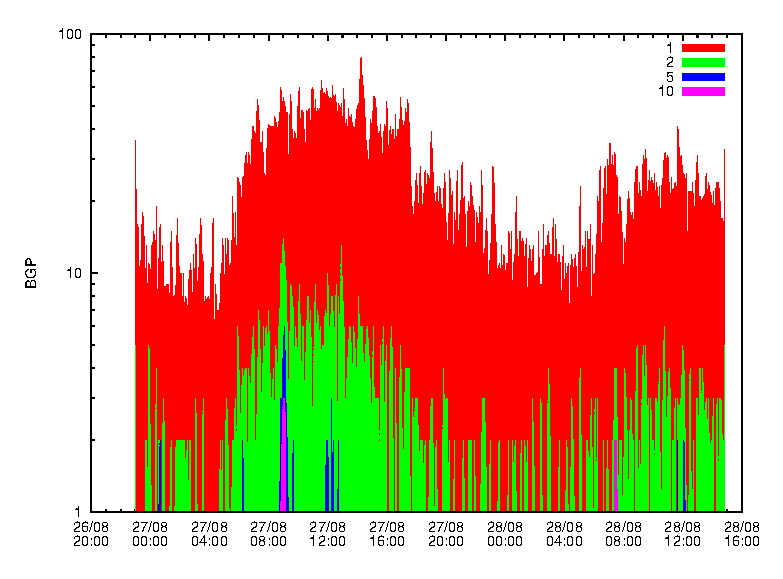
\includegraphics[width=0.75\linewidth]{images/events/2010_03_25/bgp_log_port80_ref.eps}
	\caption{Event 1: Unreachable BGP prefixes detected by the classical FACT traffic preselection based on the port-based heuristic.} 
	\label{fig:AMS_IX_FACT_REF} 
\end{figure}

\subsection{Server Socket Approach}
For evaluating the server socket bases approach, several different server socket sets are choosen, since this socket set selection process is an optimization problem as outlined in chapter \ref{chapter:integration}.

Firstly, a FACT is operated with a server socket set denoted as \emph{AllPort80SeS}, including all detected server socket listening on port 80. This socket set can directly be compared to the old heuristic approach, since it monitors a majority of those traffic as well. 

As figure \ref{fig:AMS_IX_FACT_allSES80} shows, the real event lasting from 05.00 UTC to 08:15 UTC is clearly visible equally well as in the heuristic approach from figure \ref{fig:AMS_IX_FACT_REF}. However, the server socket based approach reduces the red part indicating the number of unreachable prefixes affecting only a single internal user by at least an order of magnitude. Hence,  the event is now clearly standing out of the \emph{background event detection noise}.

Despite that fact, that the \emph{AllPort80SeS} set is not optimized at all, it outperformed the traditional approach in terms of noise reduction without significantly worsen the real event detection. This confirms the assumption that a high number of unreachable prefixes affecting only a single internal user is caused by malware and p2p churn.


\begin{figure}
	[p] \centering 
	\includegraphics[width=0.75\linewidth]{images/events/2010_03_25/bgp_log_allPort80SES.eps}
	\caption{Event 1: Unreachable BGP prefixes detected by the modified FACT traffic preselection based on all port 80 server sockets.} 
	\label{fig:AMS_IX_FACT_allSES80} 
\end{figure}


\begin{figure}
	[p] \centering 
	\includegraphics[width=0.75\linewidth]{images/events/2010_03_25/bgp_log_port80_Set_stab_0_vts_2.eps}
	\caption{Event 1: Unreachable BGP prefixes detected by the modified FACT traffic preselection based on all port 80 server sockets with visibility of at least 2 days.} 
	\label{fig:AMS_IX_FACT_allSES80VTS2} 
\end{figure}

\begin{figure}
	[p] \centering 
	\includegraphics[width=0.75\linewidth]{images/events/2010_03_25/bgp_log_port80_Set_stab_9_vts_2.eps}
	\caption{Event 1: Unreachable BGP prefixes detected by the modified FACT traffic preselection based on all port 80 server sockets with visibility of at least 2 days and stability ratio of at least $90\%$.} 
	\label{fig:AMS_IX_FACT_allSES80VTS2STAB9} 
\end{figure}

\begin{figure}
	[p] \centering 
	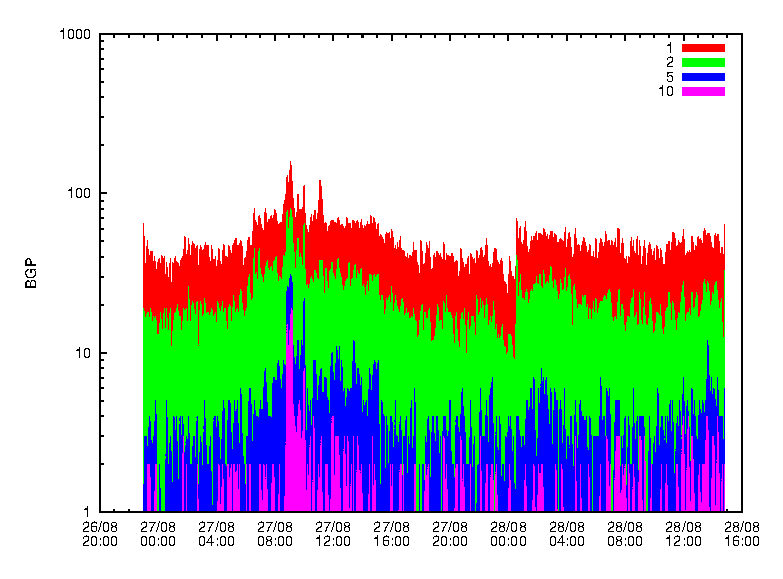
\includegraphics[width=0.75\linewidth]{images/events/2010_03_25/bgp_log_all_external.eps}
	\caption{Event 1: Unreachable BGP prefixes detected by the modified FACT traffic preselection based on all detected server sockets} 
	\label{fig:AMS_IX_FACT_allSES} 
\end{figure}

\begin{figure}
	[p] \centering 
	\includegraphics[width=0.75\linewidth]{images/events/2010_03_25/bgp_log_Set_var_0_1_stab_9_vts_2.eps}
	\caption{Event 1: Unreachable BGP prefixes detected by the modified FACT traffic preselection based on the $70\%$ most popular server sockets limited to those with a visibility of at least 2 days and stability ratio of at least $90\%$.} 
	\label{fig:AMS_IX_FACT_popularVTS2STAB9} 
\end{figure}


%%%%%%%%%%%%%%%%%%%%%%%%%%%%%%%%%%%%%%%%%%%%%%%%%%%%%%%%%%%%%%%%%%%%%%%%%%%%%%%%
% EVENT 2: TIER-1 BLACK-HOLING
%%%%%%%%%%%%%%%%%%%%%%%%%%%%%%%%%%%%%%%%%%%%%%%%%%%%%%%%%%%%%%%%%%%%%%%%%%%%%%%%
\newpage
\section{Event 2: Reverse path traffic black-holing}

On May 18, 2010, the operators of the SWITCH network were assigned to investigate an reported issue that all services in an external /24 network were not accessible from the SWITCH network between 08:30 and 08:45 UTC. According to SWITCH, the problem was most likely due to an issue of an tier-1 provider which black-holed parts of the reverse traffic towards the SWITCH network\citep{SchatzmannPAM2011}.

Unfortunately, the operators were neither able to tell how many internal users were affected nor how many external networks were unreachable during this period of time. However with the help of FACT, this issue can be further assessed with respect to the severity of the event\citep{SchatzmannPAM2011}.

\subsection{Heuristic Approach}

\begin{figure}
	[p] \centering 
	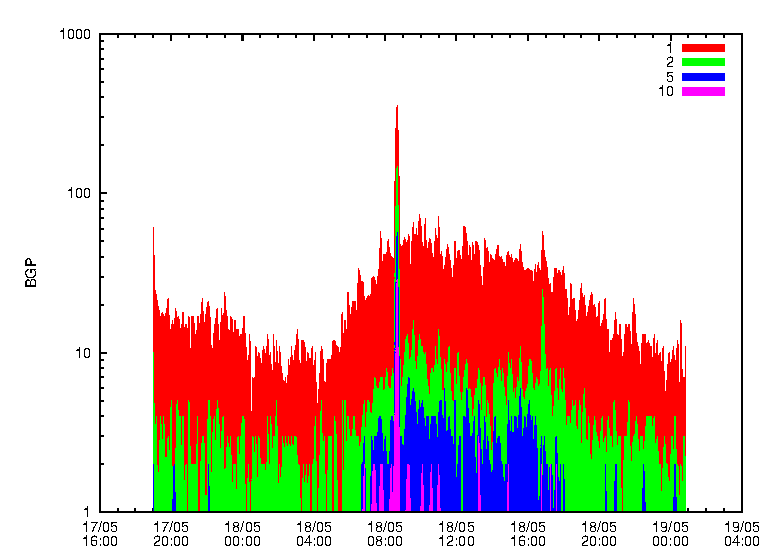
\includegraphics[width=0.75\linewidth]{images/events/2010_05_18/bgp_log_port80_ref.eps}
	\caption{Event 2: Unreachable BGP prefixes detected by the classical FACT traffic preselection based on the port-based heuristic.} 
	\label{fig:TIER1_FACT_REF} 
\end{figure}

\subsection{Server Socket Approach}

\begin{figure}
	[p] \centering 
	\includegraphics[width=0.75\linewidth]{images/events/2010_05_18/bgp_log_allPort80SES.eps}
	\caption{Event 2: Unreachable BGP prefixes detected by the modified FACT traffic preselection based on all port 80 server sockets.} 
	\label{fig:TIER1_FACT_allSES80} 
\end{figure}


\begin{figure}
	[p] \centering 
	\includegraphics[width=0.75\linewidth]{images/events/2010_05_18/bgp_log_port80_Set_stab_0_vts_2.eps}
	\caption{Event 2: Unreachable BGP prefixes detected by the modified FACT traffic preselection based on all port 80 server sockets with visibility of at least 2 days.} 
	\label{fig:TIER1_FACT_allSES80VTS2} 
\end{figure}

\begin{figure}
	[p] \centering 
	\includegraphics[width=0.75\linewidth]{images/events/2010_05_18/bgp_log_port80_Set_stab_9_vts_2.eps}
	\caption{Event 2: Unreachable BGP prefixes detected by the modified FACT traffic preselection based on all port 80 server sockets with visibility of at least 2 days and stability ratio of at least $90\%$.} 
	\label{fig:TIER1_FACT_allSES80VTS2STAB9} 
\end{figure}

\begin{figure}
	[ht] \centering 
	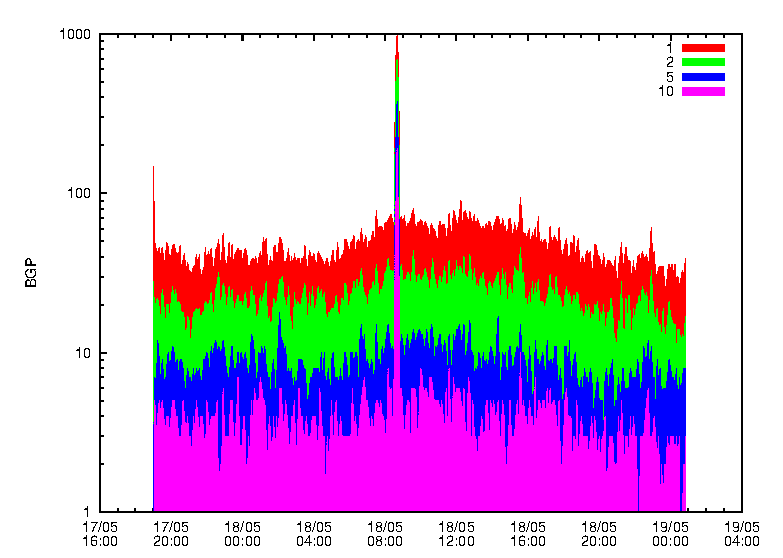
\includegraphics[width=0.75\linewidth]{images/events/2010_05_18/bgp_log_all_external.eps}
	\caption{Event 2: Unreachable BGP prefixes detected by the modified FACT traffic preselection based on all detected server sockets} 
	\label{fig:TIER1_FACT_allSES} 
\end{figure}


\begin{figure}
	[ht] \centering 
	\includegraphics[width=0.75\linewidth]{images/events/2010_05_18/bgp_log_Set_var_0_1_stab_9_vts_2.eps}
	\caption{Event 2: Unreachable BGP prefixes detected by the modified FACT traffic preselection based on the $70\%$ most popular server sockets limited to those with a visibility of at least 2 days and stability ratio of at least $90\%$.} 
	\label{fig:TIER1_FACT_popularVTS2STAB9} 
\end{figure}

%%%%%%%%%%%%%%%%%%%%%%%%%%%%%%%%%%%%%%%%%%%%%%%%%%%%%%%%%%%%%%%%%%%%%%%%%%%%%%%%
% EVENT 3: RIPE / DUKE BGP EXPERIMENT
%%%%%%%%%%%%%%%%%%%%%%%%%%%%%%%%%%%%%%%%%%%%%%%%%%%%%%%%%%%%%%%%%%%%%%%%%%%%%%%%
\newpage
\section{Event 3: RIPE / DUKE BGP Experiments}

An experiment with new BGP attributes jointly performed by RIPE and the Duke 
University on August 27, 2010, resulted in several unreachable prefixes\citep{SchatzmannPAM2011}. These 
new kind of attributes has never been announced on the Internet before,  
although it was in accordance with the BGP specification\citep{ripe_duke}.

These new kind of attributes uncovered and triggered a bug in some Cisco BGP 
Routers known as the \emph{Cisco IOS XR Software Border Gateway Protocol Vulnerability (SA-20100827-BGP)}\citep{cisco_vulnerability}. In particular, the announcements with the new attributes were corrupted 
by the Cisco Routers and send to their peers. Consequently, their peers detected 
the corruption and dropped the entire peering session\citep{ripe_duke}.

\subsection{Heuristic Approach}

\subsection{Server Socket Approach}


%!TEX root = ./main.tex
\chapter{Conclusion\label{Conclusion}}

\section{Conclusion}



\section{Future Work}
% characterize ses by time based activity (night / day, working week, weekend etc.)

% smarter socket set selection => density of network by choosing only the popularst sockets of each network

% automatization of process => danger of excluding sockets affected by events
% => consider full last week?  

% general optimization problem solving approach as simulated annealing => limit number of sockets => pareto front of sockets

% consider different selection methods as clustering analysis approaches, e.g. k-means etc => distance function include also network considerations.. etc. 

% near future public release of FlowBox and FACT



% LIST of Figures and Tables
\listoffigures
\listoftables

% Appendix-mode in Latex
\appendix

% Set enumeration to alphabetical  characters.
\renewcommand{\thepart}{\Alph{part}}
%!TEX root = ./main.tex

\chapter{Appendix}
\label{appendix}
\section{Prefix Files for FACT}

Switchextract is a neat little perl script for generating the required prefix files for the FilterInOut and the Analyser of FACT. It may be found in the tool folder of the FACT sourcecode. For correctly using these perl script, the following preliminary work have to be done:
\begin{enumerate}
	\item Download and install bgpdump from the RIPE RIS project.
	\item Download the bgpdump file of the desired date from a suitable route collector - the best from the default free rrc00.ripe.net.
	\item Adjust your own AS number within the perl script switchextract.pl, i.e. replace 559 at line 24 with your own AS number.
\end{enumerate}

Then the following steps must be executed:
\begin{enumerate}
	\item Create a file bgpdump.txt with bgpdump: \newline\texttt{bgpdump bview.XXXXXX.XXXX.gz -m > bgpdump.txt}
	\item Call the perl script switchextract.pl: \newline\texttt{perl switchextract.pl bgpdump.txt prefixes.txt}
	\item prefixes.txt has to be moved or linked to the analyser configuration folder of FACT
	\item switch\_prefixes.txt is needed by the FilterInOut and has to be moved or linked to the configuration folder of FilterInOut.
\end{enumerate}


%** Originalproblem.tex: The problem statement you received.
%!TEX root = ./main.tex

\section{Orginal Problem}

\includegraphics[width=\textwidth, page=1]{ThesisDescription.pdf}
\newpage
\includegraphics[width=\textwidth, page=2]{ThesisDescription.pdf}
\newpage
\includegraphics[width=\textwidth, page=3]{ThesisDescription.pdf}

%!TEX root = ./main.tex
\bibliographystyle{apalike} 
\bibliography{95_bib}




%!TEX root = ./main.tex
\chapter*{Eigenständigkeitserklärung} Ich erkläre hiermit, dass es sich bei
der von mir eingereichten schriftlichen Arbeit mit dem Titel
\textbf{"Who turned off the Internet? Mining Temporary Unreachability"} um eine von mir selbständig und in eigenen Worten verfasste
Originalarbeit handelt.\\

\vspace{5mm} \textbf{Verfasser:}\\
Daniel Aschwanden\\

\vspace{5mm} \textbf{Betreuer:}\\
Dominik Schatzmann\\
Dr. Bernhard Ager\\

\vspace{5mm} Mit meiner Unterschrift bestätige ich, dass ich über fachübliche
Zitierregeln unterrichtet worden bin und das Merkblatt
(\url{http://www.ethz.ch/students/exams/plagiarism_s_de.pdf}) gelesen und
verstanden habe. Die im betroffenen Fachgebiet üblichen Zitiervorschriften sind
eingehalten worden.
Eine Überprüfung der Arbeit auf Plagiate mithilfe elektronischer Hilfsmittel
darf vorgenommen werden.\\

\vspace{15mm} 
\begin{tabular}
	{l p{0.3
	\textwidth} r} Zürich, 17.10.2012 &&
	Daniel Aschwanden \\
\end{tabular}

\vfil

\end{document}

%%% Local Variables:
%%% mode: latex
%%% TeX-master: "documentation"
%%% End: